\documentclass{article}
\usepackage{iclr2027_conference,times}
%%%%% NEW MATH DEFINITIONS %%%%%

\usepackage{amsmath,amsfonts,bm}

% Mark sections of captions for referring to divisions of figures
\newcommand{\figleft}{{\em (Left)}}
\newcommand{\figcenter}{{\em (Center)}}
\newcommand{\figright}{{\em (Right)}}
\newcommand{\figtop}{{\em (Top)}}
\newcommand{\figbottom}{{\em (Bottom)}}
\newcommand{\captiona}{{\em (a)}}
\newcommand{\captionb}{{\em (b)}}
\newcommand{\captionc}{{\em (c)}}
\newcommand{\captiond}{{\em (d)}}

% Highlight a newly defined term
\newcommand{\newterm}[1]{{\bf #1}}


% Figure reference, lower-case.
\def\figref#1{figure~\ref{#1}}
% Figure reference, capital. For start of sentence
\def\Figref#1{Figure~\ref{#1}}
\def\twofigref#1#2{figures \ref{#1} and \ref{#2}}
\def\quadfigref#1#2#3#4{figures \ref{#1}, \ref{#2}, \ref{#3} and \ref{#4}}
% Section reference, lower-case.
\def\secref#1{section~\ref{#1}}
% Section reference, capital.
\def\Secref#1{Section~\ref{#1}}
% Reference to two sections.
\def\twosecrefs#1#2{sections \ref{#1} and \ref{#2}}
% Reference to three sections.
\def\secrefs#1#2#3{sections \ref{#1}, \ref{#2} and \ref{#3}}
% Reference to an equation, lower-case.
\def\eqref#1{equation~\ref{#1}}
% Reference to an equation, upper case
\def\Eqref#1{Equation~\ref{#1}}
% A raw reference to an equation---avoid using if possible
\def\plaineqref#1{\ref{#1}}
% Reference to a chapter, lower-case.
\def\chapref#1{chapter~\ref{#1}}
% Reference to an equation, upper case.
\def\Chapref#1{Chapter~\ref{#1}}
% Reference to a range of chapters
\def\rangechapref#1#2{chapters\ref{#1}--\ref{#2}}
% Reference to an algorithm, lower-case.
\def\algref#1{algorithm~\ref{#1}}
% Reference to an algorithm, upper case.
\def\Algref#1{Algorithm~\ref{#1}}
\def\twoalgref#1#2{algorithms \ref{#1} and \ref{#2}}
\def\Twoalgref#1#2{Algorithms \ref{#1} and \ref{#2}}
% Reference to a part, lower case
\def\partref#1{part~\ref{#1}}
% Reference to a part, upper case
\def\Partref#1{Part~\ref{#1}}
\def\twopartref#1#2{parts \ref{#1} and \ref{#2}}

\def\ceil#1{\lceil #1 \rceil}
\def\floor#1{\lfloor #1 \rfloor}
\def\1{\bm{1}}
\newcommand{\train}{\mathcal{D}}
\newcommand{\valid}{\mathcal{D_{\mathrm{valid}}}}
\newcommand{\test}{\mathcal{D_{\mathrm{test}}}}

\def\eps{{\epsilon}}


% Random variables
\def\reta{{\textnormal{$\eta$}}}
\def\ra{{\textnormal{a}}}
\def\rb{{\textnormal{b}}}
\def\rc{{\textnormal{c}}}
\def\rd{{\textnormal{d}}}
\def\re{{\textnormal{e}}}
\def\rf{{\textnormal{f}}}
\def\rg{{\textnormal{g}}}
\def\rh{{\textnormal{h}}}
\def\ri{{\textnormal{i}}}
\def\rj{{\textnormal{j}}}
\def\rk{{\textnormal{k}}}
\def\rl{{\textnormal{l}}}
% rm is already a command, just don't name any random variables m
\def\rn{{\textnormal{n}}}
\def\ro{{\textnormal{o}}}
\def\rp{{\textnormal{p}}}
\def\rq{{\textnormal{q}}}
\def\rr{{\textnormal{r}}}
\def\rs{{\textnormal{s}}}
\def\rt{{\textnormal{t}}}
\def\ru{{\textnormal{u}}}
\def\rv{{\textnormal{v}}}
\def\rw{{\textnormal{w}}}
\def\rx{{\textnormal{x}}}
\def\ry{{\textnormal{y}}}
\def\rz{{\textnormal{z}}}

% Random vectors
\def\rvepsilon{{\mathbf{\epsilon}}}
\def\rvtheta{{\mathbf{\theta}}}
\def\rva{{\mathbf{a}}}
\def\rvb{{\mathbf{b}}}
\def\rvc{{\mathbf{c}}}
\def\rvd{{\mathbf{d}}}
\def\rve{{\mathbf{e}}}
\def\rvf{{\mathbf{f}}}
\def\rvg{{\mathbf{g}}}
\def\rvh{{\mathbf{h}}}
\def\rvu{{\mathbf{i}}}
\def\rvj{{\mathbf{j}}}
\def\rvk{{\mathbf{k}}}
\def\rvl{{\mathbf{l}}}
\def\rvm{{\mathbf{m}}}
\def\rvn{{\mathbf{n}}}
\def\rvo{{\mathbf{o}}}
\def\rvp{{\mathbf{p}}}
\def\rvq{{\mathbf{q}}}
\def\rvr{{\mathbf{r}}}
\def\rvs{{\mathbf{s}}}
\def\rvt{{\mathbf{t}}}
\def\rvu{{\mathbf{u}}}
\def\rvv{{\mathbf{v}}}
\def\rvw{{\mathbf{w}}}
\def\rvx{{\mathbf{x}}}
\def\rvy{{\mathbf{y}}}
\def\rvz{{\mathbf{z}}}

% Elements of random vectors
\def\erva{{\textnormal{a}}}
\def\ervb{{\textnormal{b}}}
\def\ervc{{\textnormal{c}}}
\def\ervd{{\textnormal{d}}}
\def\erve{{\textnormal{e}}}
\def\ervf{{\textnormal{f}}}
\def\ervg{{\textnormal{g}}}
\def\ervh{{\textnormal{h}}}
\def\ervi{{\textnormal{i}}}
\def\ervj{{\textnormal{j}}}
\def\ervk{{\textnormal{k}}}
\def\ervl{{\textnormal{l}}}
\def\ervm{{\textnormal{m}}}
\def\ervn{{\textnormal{n}}}
\def\ervo{{\textnormal{o}}}
\def\ervp{{\textnormal{p}}}
\def\ervq{{\textnormal{q}}}
\def\ervr{{\textnormal{r}}}
\def\ervs{{\textnormal{s}}}
\def\ervt{{\textnormal{t}}}
\def\ervu{{\textnormal{u}}}
\def\ervv{{\textnormal{v}}}
\def\ervw{{\textnormal{w}}}
\def\ervx{{\textnormal{x}}}
\def\ervy{{\textnormal{y}}}
\def\ervz{{\textnormal{z}}}

% Random matrices
\def\rmA{{\mathbf{A}}}
\def\rmB{{\mathbf{B}}}
\def\rmC{{\mathbf{C}}}
\def\rmD{{\mathbf{D}}}
\def\rmE{{\mathbf{E}}}
\def\rmF{{\mathbf{F}}}
\def\rmG{{\mathbf{G}}}
\def\rmH{{\mathbf{H}}}
\def\rmI{{\mathbf{I}}}
\def\rmJ{{\mathbf{J}}}
\def\rmK{{\mathbf{K}}}
\def\rmL{{\mathbf{L}}}
\def\rmM{{\mathbf{M}}}
\def\rmN{{\mathbf{N}}}
\def\rmO{{\mathbf{O}}}
\def\rmP{{\mathbf{P}}}
\def\rmQ{{\mathbf{Q}}}
\def\rmR{{\mathbf{R}}}
\def\rmS{{\mathbf{S}}}
\def\rmT{{\mathbf{T}}}
\def\rmU{{\mathbf{U}}}
\def\rmV{{\mathbf{V}}}
\def\rmW{{\mathbf{W}}}
\def\rmX{{\mathbf{X}}}
\def\rmY{{\mathbf{Y}}}
\def\rmZ{{\mathbf{Z}}}

% Elements of random matrices
\def\ermA{{\textnormal{A}}}
\def\ermB{{\textnormal{B}}}
\def\ermC{{\textnormal{C}}}
\def\ermD{{\textnormal{D}}}
\def\ermE{{\textnormal{E}}}
\def\ermF{{\textnormal{F}}}
\def\ermG{{\textnormal{G}}}
\def\ermH{{\textnormal{H}}}
\def\ermI{{\textnormal{I}}}
\def\ermJ{{\textnormal{J}}}
\def\ermK{{\textnormal{K}}}
\def\ermL{{\textnormal{L}}}
\def\ermM{{\textnormal{M}}}
\def\ermN{{\textnormal{N}}}
\def\ermO{{\textnormal{O}}}
\def\ermP{{\textnormal{P}}}
\def\ermQ{{\textnormal{Q}}}
\def\ermR{{\textnormal{R}}}
\def\ermS{{\textnormal{S}}}
\def\ermT{{\textnormal{T}}}
\def\ermU{{\textnormal{U}}}
\def\ermV{{\textnormal{V}}}
\def\ermW{{\textnormal{W}}}
\def\ermX{{\textnormal{X}}}
\def\ermY{{\textnormal{Y}}}
\def\ermZ{{\textnormal{Z}}}

% Vectors
\def\vzero{{\bm{0}}}
\def\vone{{\bm{1}}}
\def\vmu{{\bm{\mu}}}
\def\vtheta{{\bm{\theta}}}
\def\va{{\bm{a}}}
\def\vb{{\bm{b}}}
\def\vc{{\bm{c}}}
\def\vd{{\bm{d}}}
\def\ve{{\bm{e}}}
\def\vf{{\bm{f}}}
\def\vg{{\bm{g}}}
\def\vh{{\bm{h}}}
\def\vi{{\bm{i}}}
\def\vj{{\bm{j}}}
\def\vk{{\bm{k}}}
\def\vl{{\bm{l}}}
\def\vm{{\bm{m}}}
\def\vn{{\bm{n}}}
\def\vo{{\bm{o}}}
\def\vp{{\bm{p}}}
\def\vq{{\bm{q}}}
\def\vr{{\bm{r}}}
\def\vs{{\bm{s}}}
\def\vt{{\bm{t}}}
\def\vu{{\bm{u}}}
\def\vv{{\bm{v}}}
\def\vw{{\bm{w}}}
\def\vx{{\bm{x}}}
\def\vy{{\bm{y}}}
\def\vz{{\bm{z}}}

% Elements of vectors
\def\evalpha{{\alpha}}
\def\evbeta{{\beta}}
\def\evepsilon{{\epsilon}}
\def\evlambda{{\lambda}}
\def\evomega{{\omega}}
\def\evmu{{\mu}}
\def\evpsi{{\psi}}
\def\evsigma{{\sigma}}
\def\evtheta{{\theta}}
\def\eva{{a}}
\def\evb{{b}}
\def\evc{{c}}
\def\evd{{d}}
\def\eve{{e}}
\def\evf{{f}}
\def\evg{{g}}
\def\evh{{h}}
\def\evi{{i}}
\def\evj{{j}}
\def\evk{{k}}
\def\evl{{l}}
\def\evm{{m}}
\def\evn{{n}}
\def\evo{{o}}
\def\evp{{p}}
\def\evq{{q}}
\def\evr{{r}}
\def\evs{{s}}
\def\evt{{t}}
\def\evu{{u}}
\def\evv{{v}}
\def\evw{{w}}
\def\evx{{x}}
\def\evy{{y}}
\def\evz{{z}}

% Matrix
\def\mA{{\bm{A}}}
\def\mB{{\bm{B}}}
\def\mC{{\bm{C}}}
\def\mD{{\bm{D}}}
\def\mE{{\bm{E}}}
\def\mF{{\bm{F}}}
\def\mG{{\bm{G}}}
\def\mH{{\bm{H}}}
\def\mI{{\bm{I}}}
\def\mJ{{\bm{J}}}
\def\mK{{\bm{K}}}
\def\mL{{\bm{L}}}
\def\mM{{\bm{M}}}
\def\mN{{\bm{N}}}
\def\mO{{\bm{O}}}
\def\mP{{\bm{P}}}
\def\mQ{{\bm{Q}}}
\def\mR{{\bm{R}}}
\def\mS{{\bm{S}}}
\def\mT{{\bm{T}}}
\def\mU{{\bm{U}}}
\def\mV{{\bm{V}}}
\def\mW{{\bm{W}}}
\def\mX{{\bm{X}}}
\def\mY{{\bm{Y}}}
\def\mZ{{\bm{Z}}}
\def\mBeta{{\bm{\beta}}}
\def\mPhi{{\bm{\Phi}}}
\def\mLambda{{\bm{\Lambda}}}
\def\mSigma{{\bm{\Sigma}}}

% Tensor
\DeclareMathAlphabet{\mathsfit}{\encodingdefault}{\sfdefault}{m}{sl}
\SetMathAlphabet{\mathsfit}{bold}{\encodingdefault}{\sfdefault}{bx}{n}
\newcommand{\tens}[1]{\bm{\mathsfit{#1}}}
\def\tA{{\tens{A}}}
\def\tB{{\tens{B}}}
\def\tC{{\tens{C}}}
\def\tD{{\tens{D}}}
\def\tE{{\tens{E}}}
\def\tF{{\tens{F}}}
\def\tG{{\tens{G}}}
\def\tH{{\tens{H}}}
\def\tI{{\tens{I}}}
\def\tJ{{\tens{J}}}
\def\tK{{\tens{K}}}
\def\tL{{\tens{L}}}
\def\tM{{\tens{M}}}
\def\tN{{\tens{N}}}
\def\tO{{\tens{O}}}
\def\tP{{\tens{P}}}
\def\tQ{{\tens{Q}}}
\def\tR{{\tens{R}}}
\def\tS{{\tens{S}}}
\def\tT{{\tens{T}}}
\def\tU{{\tens{U}}}
\def\tV{{\tens{V}}}
\def\tW{{\tens{W}}}
\def\tX{{\tens{X}}}
\def\tY{{\tens{Y}}}
\def\tZ{{\tens{Z}}}


% Graph
\def\gA{{\mathcal{A}}}
\def\gB{{\mathcal{B}}}
\def\gC{{\mathcal{C}}}
\def\gD{{\mathcal{D}}}
\def\gE{{\mathcal{E}}}
\def\gF{{\mathcal{F}}}
\def\gG{{\mathcal{G}}}
\def\gH{{\mathcal{H}}}
\def\gI{{\mathcal{I}}}
\def\gJ{{\mathcal{J}}}
\def\gK{{\mathcal{K}}}
\def\gL{{\mathcal{L}}}
\def\gM{{\mathcal{M}}}
\def\gN{{\mathcal{N}}}
\def\gO{{\mathcal{O}}}
\def\gP{{\mathcal{P}}}
\def\gQ{{\mathcal{Q}}}
\def\gR{{\mathcal{R}}}
\def\gS{{\mathcal{S}}}
\def\gT{{\mathcal{T}}}
\def\gU{{\mathcal{U}}}
\def\gV{{\mathcal{V}}}
\def\gW{{\mathcal{W}}}
\def\gX{{\mathcal{X}}}
\def\gY{{\mathcal{Y}}}
\def\gZ{{\mathcal{Z}}}

% Sets
\def\sA{{\mathbb{A}}}
\def\sB{{\mathbb{B}}}
\def\sC{{\mathbb{C}}}
\def\sD{{\mathbb{D}}}
% Don't use a set called E, because this would be the same as our symbol
% for expectation.
\def\sF{{\mathbb{F}}}
\def\sG{{\mathbb{G}}}
\def\sH{{\mathbb{H}}}
\def\sI{{\mathbb{I}}}
\def\sJ{{\mathbb{J}}}
\def\sK{{\mathbb{K}}}
\def\sL{{\mathbb{L}}}
\def\sM{{\mathbb{M}}}
\def\sN{{\mathbb{N}}}
\def\sO{{\mathbb{O}}}
\def\sP{{\mathbb{P}}}
\def\sQ{{\mathbb{Q}}}
\def\sR{{\mathbb{R}}}
\def\sS{{\mathbb{S}}}
\def\sT{{\mathbb{T}}}
\def\sU{{\mathbb{U}}}
\def\sV{{\mathbb{V}}}
\def\sW{{\mathbb{W}}}
\def\sX{{\mathbb{X}}}
\def\sY{{\mathbb{Y}}}
\def\sZ{{\mathbb{Z}}}

% Entries of a matrix
\def\emLambda{{\Lambda}}
\def\emA{{A}}
\def\emB{{B}}
\def\emC{{C}}
\def\emD{{D}}
\def\emE{{E}}
\def\emF{{F}}
\def\emG{{G}}
\def\emH{{H}}
\def\emI{{I}}
\def\emJ{{J}}
\def\emK{{K}}
\def\emL{{L}}
\def\emM{{M}}
\def\emN{{N}}
\def\emO{{O}}
\def\emP{{P}}
\def\emQ{{Q}}
\def\emR{{R}}
\def\emS{{S}}
\def\emT{{T}}
\def\emU{{U}}
\def\emV{{V}}
\def\emW{{W}}
\def\emX{{X}}
\def\emY{{Y}}
\def\emZ{{Z}}
\def\emSigma{{\Sigma}}

% entries of a tensor
% Same font as tensor, without \bm wrapper
\newcommand{\etens}[1]{\mathsfit{#1}}
\def\etLambda{{\etens{\Lambda}}}
\def\etA{{\etens{A}}}
\def\etB{{\etens{B}}}
\def\etC{{\etens{C}}}
\def\etD{{\etens{D}}}
\def\etE{{\etens{E}}}
\def\etF{{\etens{F}}}
\def\etG{{\etens{G}}}
\def\etH{{\etens{H}}}
\def\etI{{\etens{I}}}
\def\etJ{{\etens{J}}}
\def\etK{{\etens{K}}}
\def\etL{{\etens{L}}}
\def\etM{{\etens{M}}}
\def\etN{{\etens{N}}}
\def\etO{{\etens{O}}}
\def\etP{{\etens{P}}}
\def\etQ{{\etens{Q}}}
\def\etR{{\etens{R}}}
\def\etS{{\etens{S}}}
\def\etT{{\etens{T}}}
\def\etU{{\etens{U}}}
\def\etV{{\etens{V}}}
\def\etW{{\etens{W}}}
\def\etX{{\etens{X}}}
\def\etY{{\etens{Y}}}
\def\etZ{{\etens{Z}}}

% The true underlying data generating distribution
\newcommand{\pdata}{p_{\rm{data}}}
% The empirical distribution defined by the training set
\newcommand{\ptrain}{\hat{p}_{\rm{data}}}
\newcommand{\Ptrain}{\hat{P}_{\rm{data}}}
% The model distribution
\newcommand{\pmodel}{p_{\rm{model}}}
\newcommand{\Pmodel}{P_{\rm{model}}}
\newcommand{\ptildemodel}{\tilde{p}_{\rm{model}}}
% Stochastic autoencoder distributions
\newcommand{\pencode}{p_{\rm{encoder}}}
\newcommand{\pdecode}{p_{\rm{decoder}}}
\newcommand{\precons}{p_{\rm{reconstruct}}}

\newcommand{\laplace}{\mathrm{Laplace}} % Laplace distribution

\newcommand{\E}{\mathbb{E}}
\newcommand{\Ls}{\mathcal{L}}
\newcommand{\R}{\mathbb{R}}
\newcommand{\emp}{\tilde{p}}
\newcommand{\lr}{\alpha}
\newcommand{\reg}{\lambda}
\newcommand{\rect}{\mathrm{rectifier}}
\newcommand{\softmax}{\mathrm{softmax}}
\newcommand{\sigmoid}{\sigma}
\newcommand{\softplus}{\zeta}
\newcommand{\KL}{D_{\mathrm{KL}}}
\newcommand{\Var}{\mathrm{Var}}
\newcommand{\standarderror}{\mathrm{SE}}
\newcommand{\Cov}{\mathrm{Cov}}
% Wolfram Mathworld says $L^2$ is for function spaces and $\ell^2$ is for vectors
% But then they seem to use $L^2$ for vectors throughout the site, and so does
% wikipedia.
\newcommand{\normlzero}{L^0}
\newcommand{\normlone}{L^1}
\newcommand{\normltwo}{L^2}
\newcommand{\normlp}{L^p}
\newcommand{\normmax}{L^\infty}

\newcommand{\parents}{Pa} % See usage in notation.tex. Chosen to match Daphne's book.

\DeclareMathOperator*{\argmax}{arg\,max}
\DeclareMathOperator*{\argmin}{arg\,min}

\DeclareMathOperator{\sign}{sign}
\DeclareMathOperator{\Tr}{Tr}
\let\ab\allowbreak


\usepackage{booktabs}
\usepackage{graphicx}
\usepackage{hyperref}
\usepackage{microtype}
\usepackage{url}
\usepackage{xurl}

\title{BYOD: Build Your Own DLM - Efficient Autoregressive-to-Diffusion Language Model Conversion}

% Keep the submission anonymous. Do not uncomment \iclrfinalcopy until camera ready.
\author{Anonymous authors}

\newcommand{\method}{BYOD}
\newcommand{\na}{--}

\begin{document}
\maketitle

\begin{abstract}
Unlike autoregressive (AR) models, diffusion language models (DLMs) permit parallel token updates, flexible generation, and bidirectional attention, but leading systems rely on costly pretraining or full-model fine-tuning. We present Build Your Own DLM (BYOD), a generalizable LoRA-only recipe for parameter-efficient AR-to-DLM conversion. Without architecture-specific tuning, BYOD induces diffusion generation in Gemma 2 9B, Llama 3.1 8B, Qwen2.5 7B, and Ministral 8B; to our knowledge, this is the first reported AR-to-DLM conversion of a Mistral-8B model. The adapters comprise 4.1--5.8\% of final parameters while every base-model parameter remains frozen; each 25,000-iteration conversion needs at most 102.4M tokens, processed in 3.1--4.0 hours on one Google Colab GPU. All four models generate from fully masked sequences, use bidirectional context in a controlled attention test, and retain substantial parent-model knowledge. BYOD-Gemma is the strongest BYOD conversion on our nine-task evaluation, reaching 52.4\% average accuracy compared with 49.6\% for LLaDA 8B Instruct in the same harness. Open-generation quality at low network function evaluation (NFE) budgets remains the principal limitation: BYOD perplexity is 8.3--11.1 versus 4.1 for LLaDA when generating 128 tokens in 64 steps. To enable further experimentation and inspection, we release our training and evaluation code, converted models, and accessible interactive demos upon acceptance. BYOD thus provides a practical route for extending diffusion generation to other existing model families while identifying the gap that efficient conversion must next close.

\noindent\textbf{Code:} After acceptance.\quad\textbf{BYOD demos:}
\href{https://huggingface.co/spaces/Dovelove/byod-gemma-2-9b}{Gemma} $\mid$
\href{https://huggingface.co/spaces/Dovelove/byod-llama-3.1-8b}{Llama} $\mid$
\href{https://huggingface.co/spaces/Dovelove/byod-qwen2.5-7b}{Qwen} $\mid$
\href{https://huggingface.co/spaces/Dovelove/byod-ministral-8b}{Ministral}
\end{abstract}

\section{Introduction}

Autoregressive (AR) language models generate left to right. This simple learning target scales effectively, but fixes the generation order, restricts attention to prior tokens, and produces only one new token per step. Diffusion language models (DLMs) instead iteratively reconstruct multiple positions in a corrupted sequence using bidirectional context \citep{austin2021structured,sahoo2024simple,shi2024simplified}. Their number of function evaluations (NFE) can be chosen independently of output length, and early low-probability predictions can be revised. Training or adapting models for diffusive generation, however, has remained computationally intensive and expensive.

\begin{figure*}[t!]
\centering
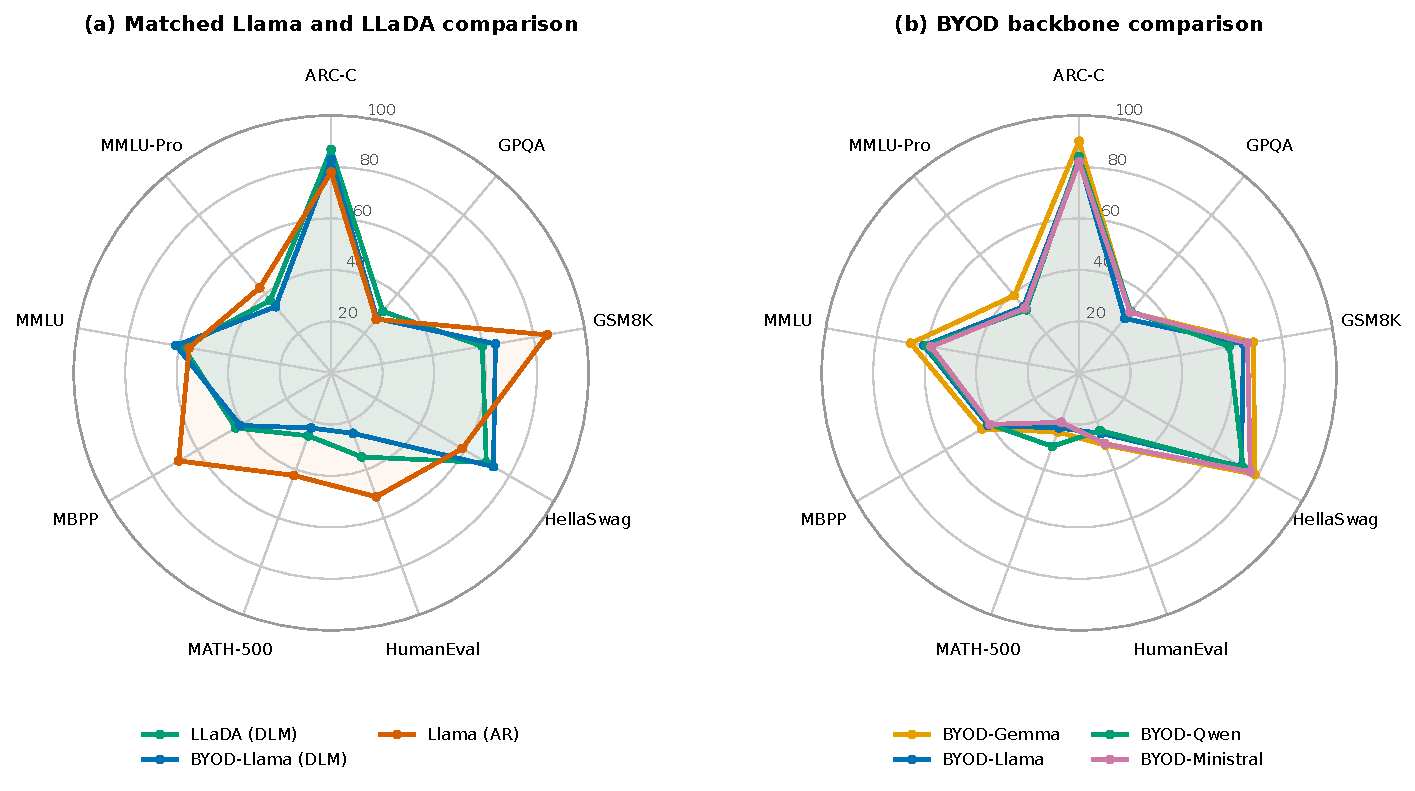
\includegraphics[width=\textwidth]{figures/benchmark_radar_panels.pdf}
\caption{Task-level accuracy profiles on the same 250 questions per task, or all 164 HumanEval questions. (a) LLaDA, BYOD-Llama-25k, and the unchanged Llama AR parent. (b) The four primary BYOD conversions. All spokes use an absolute 0--100\% scale.}
\label{fig:benchmark-radars}
\end{figure*}

Our primary aim is therefore a compute-efficient, reproducible recipe for converting AR models into DLMs without pretraining a diffusion foundation model for every architecture. This matters for three reasons. First, full diffusion pretraining is financially and environmentally costly: for example, under our standardized rental and electricity scenario, the reported LLaDA run corresponds to approximately \$675,000 and 44,100 kg CO$_2$e (Table~\ref{tab:compute}). It should be noted that these illustrative estimates are neither the authors' bill nor measured emissions; operational carbon depends strongly on utilization, datacenter efficiency, location, and energy supply \citep{strubell2019energy,patterson2021carbon}. Second, AR-to-DLM conversion in hours on one widely available cloud instance makes hands-on DLM research available beyond laboratories with multi-node clusters. Third, applying the same inexpensive intervention to multiple existing model families makes it feasible to study how architecture and parent-model choice affect diffusion generation without repeating foundation-model pretraining for every comparison.

We study this question with \method{}, a generalizable conversion and evaluation pipeline for four instruction-tuned decoder families: Gemma~2~9B, Llama~3.1~8B, Qwen2.5~7B, and Ministral~8B. We selected the latest, comparably sized text-only instruction checkpoints to avoid modality-specific confounding. Every backbone receives the same bidirectional attention intervention, LoRA target modules, and masked-diffusion objective. Comparing with each released parent makes the observed capability changes explicit. We also evaluate LLaDA~8B Instruct in the same harness as an external masked-diffusion reference with overlapping benchmarks. Its different size and training history prevent treating this as a controlled comparison of LoRA and full-parameter training. We additionally report published DiffuLLaMA, Dream-Instruct, iLLaDA-Instruct, and Efficient-DLM values, but keep them protocol-separated: their additional attention, masking, scheduling, data, and inference techniques would confound a controlled comparison.

Our contributions are:
\begin{itemize}
    \item a compute-efficient recipe that converts four instruction-tuned AR model families to masked diffusion using only a few single-GPU hours and LoRA parameter updates;
    \item a paired evaluation of each diffusion model and its frozen AR parent across general knowledge, reasoning, mathematics, and code benchmarks;
    \item a controlled analysis of training duration, denoising-step count, validation loss, perplexity and distinct n-grams; and
    \item anonymous interactive demos for all four models, with training and inference code released upon acceptance, support accessible DLM conversion and qualitative evaluation.
\end{itemize}

\section{Related work}

Discrete diffusion models corrupt and reconstruct categorical sequences rather than adding Gaussian noise. D3PM formalized categorical corruption with transition matrices, including an absorbing process in which tokens transition to a dedicated mask state \citep{austin2021structured}. MDLM and contemporaneous work showed that this masked formulation admits a simple noise-weighted cross-entropy objective, while RADD reparameterized the predictor in terms of conditional distributions over clean tokens \citep{sahoo2024simple,shi2024simplified,ou2024absorbing}. These approaches form the basis of masked diffusion language models (MDLMs). Uniform (or multinomial) diffusion, which instead corrupts tokens with samples from the ordinary vocabulary, is another option \citep{hoogeboom2021multinomial}; we use the simpler absorbing-mask denoising objective employed by LLaDA.

\begin{table*}[t]
\caption{Incremental training scale and standardized resource estimates for comparable diffusion systems. GPU-hours marked $^\dagger$ are estimated from published model/data scale; unmarked values are reported. We stress that cost and CO$_2$e are estimates purely for illustrative purposes, based on a standardized operational scenario (Appendix~\ref{app:cost}), not reported values. NR: insufficient information.}
\label{tab:compute}
\centering
\scriptsize
\resizebox{\textwidth}{!}{%
\begin{tabular}{llllrrr}
\toprule
System & Diffusion-stage data & Updated weights & Hardware & GPU-h & Cost (USD) & CO$_2$e \\
\midrule
\method{} (ours) & $\leq$102.4M tokens & LoRA & 1$\times$RTX Pro 6000 & 3.2 & \$11 & 0.9 kg \\
DiffuLLaMA 7B & 65B tokens & Full & 64$\times$GH200 & 1,917$^\dagger$ & \$9,951 & 0.65 t \\
LLaDA 8B & 2.3T tokens & Full & H800 & 130,000 & \$674,830 & 44.1 t \\
Dream 7B & 580B tokens + SFT & Full & NR & 17,105$^\dagger$ & \$88,791 & 5.81 t \\
iLLaDA 8B & 12T tokens + SFT & Full & NR & 404,449$^\dagger$ & \$2,099,494 & 137.3 t \\
Efficient-DLM 8B & 500B tokens & Full & 128$\times$H100 & 16,852$^\dagger$ & \$87,479 & 5.72 t \\
Uno 8B & 7B tokens & LoRA & 64$\times$H200 & 3,840 & \$19,933 & 1.30 t \\
Fast-dLLM v2 7B & $\sim$1B tokens & Full & 64$\times$A100 & 768 & \$3,987 & 149 kg \\
\bottomrule
\end{tabular}}
\end{table*}

The authors of LLaDA were the first to scale masked diffusion to an 8B general-purpose language model \citep{nie2025llada}. Its architecture follows Llama~3.1~8B, but it was pretrained from scratch using 2.3T tokens and 130,000 GPU-hours. AR-to-diffusion conversion instead reuses knowledge from an AR checkpoint. DiffuLLaMA established this route through 65B tokens of full-model continued training at 7B scale \citep{gong2025diffullama}. Dream uses DiffuLLaMA's shifted-prediction initialization, continues Qwen2.5 for 580B tokens, and adds context-adaptive token-level noise rescheduling \citep{ye2025dream}. Efficient-DLM combines 500B tokens of continued training with blockwise attention and position-dependent masking \citep{fu2025efficientdlm}, whereas iLLaDA uses from-scratch diffusion pretraining at substantially larger scale \citep{nie2026illada}. Conversion has also reached larger sparse models through RND1 (30B parameters), LLaDA2.0 (16B and 100B), and DiffusionGemma (25.2B, using uniform diffusion) \citep{chandrasegaran2025rnd1,bie2025llada20,diffusiongemma2026}. Thus, Gemma-, Llama-, and Qwen-based diffusion models were already reported, but we found no prior diffusion conversion of Ministral~8B Instruct~2410.

Hybrid and blockwise models offer a different compromise between bidirectionality and deployability. Block Diffusion is autoregressive across blocks but diffusive within each block, enabling variable-length generation and inter-block KV caching \citep{arriola2025block}. Fast-dLLM v2 converts Qwen2.5 models using full-parameter fine-tuning with approximately 1B tokens and combines blockwise complementary masking with hierarchical caching \citep{wu2025fastdllmv2}. These systems retain more left-to-right structure than our fully bidirectional answer block, making them especially relevant to speed, caching, and arbitrary-length generation but not suited as direct controls for our intervention.

LAD showed that LoRA and bidirectional attention can induce diffusion-style generation, combining masking with token swaps, duplications, and span shifts \citep{kuiper2025lad,hu2022lora}. \method{} builds on that adaptation mechanism, rather than introducing LoRA-based conversion itself. LAD tested three sizes within the Llama family; \method{} tests whether a shared IID absorbing-mask recipe transfers across four model families. Appendix~\ref{app:lad-comparison} compares published LAD and BYOD-Llama benchmark results, with their different evaluation protocols stated explicitly. Other LoRA-based diffusion work addresses different goals: Uno learns diffusion-draft adapters while retaining the AR model as verifier, the dLLM framework uses LoRA to fine-tune already-diffusive checkpoints rather than for its Tiny-A2D conversion, and NaRA adapts existing diffusion models with noise-conditioned LoRA \citep{sahoo2026uno,zhou2026dllm,wang2026nara}. Thus, their LoRA components augment already diffusively generating models, rather than converting AR model families into standalone diffusion models.

Table~\ref{tab:compute} compares training budgets for similarly sized diffusion models. For AR-to-diffusion conversion methods, these budgets exclude the substantial earlier cost of training the AR parent; for from-scratch methods they include diffusion pretraining. Dollar and operational-emissions columns are rental-equivalent estimates under one documented pricing and energy scenario, not the authors' actual bills or measured footprints; Appendix~\ref{app:cost} gives the complete calculation and its limitations.

Our study has explicitly chosen to hold the adaptation mechanism as constant as the architectures permit, repeat it across four families, and benchmark each converted model against the exact AR checkpoint from which it originated. This paired comparison is essential because it allows us to compare our results directly with the prior capability of the parent model.

\section{Method}

\subsection{Masked-diffusion training objective}

The training objective teaches the adapted model to reconstruct masked response tokens while conditioning on an uncorrupted instruction.

Let $p$ be the instruction, $x_0=(x_0^1,\ldots,x_0^L)$ the clean response region, $A$ the answer positions, and $P$ the EOS-padding positions. For each example, we sample $t\sim\mathcal{U}[10^{-3},1]$ and independently mask each position in $A\cup P$ with probability $t$, yielding the corrupted sequence $x_t$ and masked set $M_t$. For either region $R\in\{A,P\}$, we calculate the same-position reconstruction loss
\begin{equation}
\ell_R(\theta)=-\frac{1}{t|R|}
\sum_{i\in M_t\cap R}
\log p_{\phi,\theta}(x_0^i\mid p,x_t).
\label{eq:region-loss}
\end{equation}
We then combine the answer and padding losses:
\begin{equation}
\mathcal{L}(\theta)=\mathbb{E}_{t,x_0,x_t}
\left[0.9\ell_A(\theta)+0.1\ell_P(\theta)\right].
    \label{eq:objective}
\end{equation}
Here, $p_{\phi,\theta}$ is the conditional token distribution, $\phi$ denotes the frozen parent parameters, and $\theta$ the LoRA parameters. The first terminating EOS is included as a genuine answer token; all subsequent EOS tokens are treated as padding. The factor $1/t$ corrects for the sampled masking rate. Prompt and chat-template tokens remain visible to the model and are not part of the loss. Training masks are resampled online; validation masks are fixed by example index and seed.

\begin{table}[t]
\caption{Diffusion model names matched to parent models, their trainable parameter counts, and measured time for 25,000 updates. All trainable parameters are rank-1024 Q/V LoRA weights.}
\label{tab:models}
\centering
\small
\resizebox{\columnwidth}{!}{%
\begin{tabular}{llrrrr}
\toprule
Diffusion model & AR parent & Total parameters & Trainable & Trainable (\%) & Time (h) \\
\midrule
BYOD-Gemma & Gemma 2 9B IT & 10.732B & 572.5M & 5.33 & 4.0 \\
BYOD-Qwen & Qwen2.5 7B Instruct & 7.939B & 323.0M & 4.07 & 3.1 \\
BYOD-Ministral & Ministral 8B Instruct 2410 & 8.511B & 490.7M & 5.77 & 3.4 \\
BYOD-Llama & Llama 3.1 8B Instruct & 8.466B & 436.2M & 5.15 & 3.2 \\
\bottomrule
\end{tabular}}
\end{table}

\subsection{Autoregressive-to-diffusion conversion}

To convert an autoregressive model to a diffusion-style model, we replace the causal mask in every layer with a bidirectional attention mask, so every prompt, answer, and EOS-padding position can attend to every position. We attach LoRA adapters to every self-attention query and value projection, with rank $r=1024$, scaling $\alpha=1024$, and dropout zero. The rest of the model architecture and output vocabulary remain unchanged. Backbone weights, token embeddings, the language-model head, biases, and normalization layers are frozen. The pretrained output head is also retained unchanged: whereas autoregressive training compares each position’s logits with the next token through shifted labels, BYOD removes this label shift and predicts the clean token at the same position from the bidirectionally attended, corrupted sequence. Each model reuses an existing single-token string from its tokenizer (\texttt{MASK} for Gemma, Llama, and Qwen; \texttt{<?>} for Ministral), avoiding vocabulary expansion.

We fix the LoRA rank across model families to retain one architecture-independent recipe. Matching trainable parameter counts would require model-specific ranks and would still not control for differences in depth, width, and attention design. This results in variation in trainable parameters, which is therefore a potential confounder in cross-family comparisons. Every conversion was trained on one NVIDIA RTX PRO 6000 GPU in Google Colab, without distributed parallelism; Table~\ref{tab:models} reports parameter counts and conversion times. A separate rank ablation on Llama examines validation loss and training-update cost under fixed settings (Appendix~\ref{app:rank-ablation}).

For deployment, each adapter can be folded into its parent projection as $W_{\mathrm{merged}}=W+(\alpha/r)BA$, where $W$ is the frozen projection and $A$ and $B$ are the learned low-rank matrices. This removes the adapter branch while retaining the bidirectional attention intervention. Appendix~\ref{app:merge} evaluates whether merging changes model behavior.

\subsection{Training data}

We construct a one-million-example mixture containing 45\% general instruction following, 18\% multiple-choice reasoning, 18\% mathematics, and 19\% code. Within these groups, the source weights are: Clean-Instruct-3M/T\"ulu~3/Alpaca-GPT4/Alpaca at 40/35/20/5 \citep{cleaninstruct3m,lambert2024tulu3,peng2023instructiongpt4,taori2023alpaca}; MMLU/HellaSwag/ARC-Easy at 73/25/2 \citep{hendrycks2021mmlu,zellers2019hellaswag,clark2018arc}; Orca-Math/GSM8K at 95/5 \citep{mitra2024orcamath,cobbe2021gsm8k}; and OpenCoder/MBPP at 99.7/0.3 \citep{huang2024opencoder,austin2021mbpp}. When applicable, only the training splits are used. We deduplicate normalized prompts, exclude exact matches with held-out benchmark prompts, and retain only examples that fit the 256-token training length. Each model receives the same shuffled examples, retokenized with its native chat template and tokenizer. Prompt tokens remain clean; only answer and EOS-padding positions can be corrupted.

The four primary models see the same dataset prefix. BYOD-Llama-50k uses the same fixed shuffle for a longer, 800,000-example run with newly sampled corruptions. Exact run sizes and optimization settings are given in Appendix~\ref{app:training-settings}.

\subsection{Inference}
Inference begins from a fixed-length, fully masked answer block. At each denoising step, the model predicts all masked positions, retains the most confident predictions, and remasks lower-confidence positions; accepted tokens remain unmasked. This can resolve several output tokens per network evaluation. Task-specific lengths, denoising budgets, temperatures, and EOS/EOT handling are given in Appendix~\ref{app:inference-settings}.

\begin{figure}[t]
\centering
\fbox{\begin{minipage}{0.92\columnwidth}
\small
\textbf{User:} Replace the masked token in the partial assistant response with exactly the word written after ``COPY:''. Copy the spelling exactly. Do not use a synonym or a related word.\par\smallskip
\textbf{Initial masked model input:}\par
\texttt{Answer: [MASK]. COPY: apple.}\par\smallskip
\textbf{Expected model response:}\par
\texttt{Answer: apple. COPY: apple.}
\end{minipage}}
\caption{Example input and expected reconstruction for the bidirectional attention test. Only the masked position is predicted.}
\label{fig:bidirectional-example}
\end{figure}

\section{Evaluation}
\subsection{Paired models and baselines}
We refer to the four conversions as BYOD-Gemma, BYOD-Qwen, BYOD-Ministral, and BYOD-Llama. For Llama, we distinguish the primary and longer-trained checkpoints as BYOD-Llama-25k and BYOD-Llama-50k. We also compare each model with its unchanged AR parent. LLaDA~8B Instruct serves as an external diffusion baseline in the same harness; results reported by other papers are presented separately because their protocols differ. We specifically use BYOD-Llama for the longer run and checkpoint-wise analysis because DiffuLLaMA, LLaDA, and iLLaDA use Llama or closely related Llama-style architectures, making it the clearest basis for comparison with prominent general-purpose DLMs \citep{gong2025diffullama,nie2025llada,nie2026illada}. We also compare BYOD-Llama-25k before and after folding its LoRA weights into the base model, to see if merging deteriorates the results. The nine standard task benchmarks use greedy token selection and low-confidence remasking, while open-ended generation uses temperature 0.7 and delayed EOS/EOT acceptance. Complete settings are reported in Appendix~\ref{app:inference-settings}.

\subsection{Task benchmarks}
Our benchmark set contains MMLU, MMLU-Pro, HellaSwag, ARC-Challenge, GSM8K, MATH-500, GPQA-Main, HumanEval, and sanitized MBPP \citep{hendrycks2021mmlu,wang2024mmlupro,zellers2019hellaswag,clark2018arc,cobbe2021gsm8k,hendrycks2021math,rein2023gpqa,chen2021codex,austin2021mbpp}. We evaluate the same 250 questions per task across all ten model/checkpoint configurations, except HumanEval, where we use all 164 questions. This gives 2,164 questions per configuration and 21,640 model--question outcomes. Appendix~\ref{app:benchmark-uncertainty} lists the evaluation splits, available set sizes and full results with uncertainty intervals. We score multiple-choice tasks by option label, GSM8K by its final number, MATH by normalized final-answer equivalence with symbolic verification, and code tasks by whether the generated program passes the supplied tests in an isolated subprocess.

The overall score is the equal-weight mean of the nine task accuracies. We report nominal 95\% intervals for these means using 20,000 bootstrap resamples of questions within each task, keeping the tasks fixed. Intervals for model differences use paired resampling of the same questions for both models. These intervals are not adjusted for comparing several model configurations or selecting the strongest observed conversion, and we do not use them to claim superiority. Per-task Wilson intervals appear in Appendix~\ref{app:benchmark-uncertainty}; these estimates describe item variation, not variation across training runs.

\subsection{Open-ended generation}
We assess output fluency with perplexity and Distinct-1/2/3 calculated over answers on 100 open-ended questions. Standard masked diffusion does not directly provide the left-to-right sequence likelihood used for AR perplexity, and its usual evidence lower bound is not a proper test-time likelihood \citep{turok2026duel}. We therefore follow prior DLM work and use frozen Microsoft Phi-4 14B as an external perplexity scorer \citep{gong2025diffullama}. We pool negative log-likelihoods across all non-padding tokens of all generated answers before exponentiating, so every token has equal weight. Because this score does not measure diversity, we also report sliding model-token Distinct-1/2/3 percentages after removing special tokens. Higher Distinct-$n$ indicates less local repetition \citep{li2016diversity}; in our experiments, it exposed cases where perplexity improved because output became more repetitive rather than better.

\subsection{Bidirectional attention test}
We test whether the converted diffusion models allow bidirectional information flow with a simple right-context copy task (Appendix~\ref{app:bidirectional-infilling}). Most of the response is pre-filled, and the model must fill an earlier masked position by copying a word shown later in the response. A causal model cannot change its prediction at an earlier position based on a later token, so sensitivity to this clue directly tests functional bidirectional attention. Figure~\ref{fig:bidirectional-example} shows one test item and its expected reconstruction.

\section{Results}

\subsection{Benchmark accuracy and base-model dependence}

\begin{table*}[t]
\caption{Accuracy (\%) in our common harness: 250 shared questions per task, or all 164 HumanEval questions. D is a converted diffusion model; AR is its unchanged parent. Llama D-25k and D-50k share the same parent. Bold marks the best observed common-harness diffusion score; underline marks the best observed BYOD score (ties retained). The average gives each task equal weight; its nominal, unadjusted 95\% bootstrap interval appears below it. Published LLaDA scores use a separate protocol and have no interval computed here. AR has intentionally longer output limits (Appendix~\ref{app:inference-settings}). Full per-task intervals appear in Appendix~\ref{app:benchmark-uncertainty}.}
\label{tab:accuracy}
\centering
\scriptsize
\setlength{\tabcolsep}{2pt}
\resizebox{\textwidth}{!}{%
% Generated by analysis/update_manuscript_benchmarks.py; do not edit values by hand.
\begin{tabular}{lrrrrrrrrrrr}
\toprule
& \multicolumn{2}{c}{Gemma} & \multicolumn{2}{c}{Qwen} & \multicolumn{2}{c}{Ministral} & \multicolumn{3}{c}{Llama} & \multicolumn{2}{c}{LLaDA} \\
Task & D & AR & D & AR & D & AR & D-25k & D-50k & AR & Ours & Published \\
\midrule
ARC-C & \textbf{\underline{90.0}} & 88.8 & 84.0 & 90.0 & 82.0 & 72.0 & 82.8 & 81.6 & 78.0 & 86.8 & 88.5 \\
GPQA & 30.8 & 29.6 & \textbf{\underline{31.2}} & 33.6 & 30.8 & 32.4 & 27.6 & 28.0 & 27.2 & \textbf{31.2} & 33.3 \\
HellaSwag & \textbf{\underline{78.8}} & 70.4 & 73.6 & 74.4 & 76.8 & 72.4 & 72.8 & 77.2 & 58.8 & 69.6 & 74.6 \\
MMLU & \textbf{\underline{66.4}} & 65.6 & 60.4 & 69.2 & 58.4 & 54.8 & 61.2 & 60.0 & 56.0 & 58.4 & 65.5 \\
MMLU-Pro & \textbf{\underline{39.2}} & 44.4 & 32.0 & 46.4 & 32.8 & 35.6 & 33.6 & 31.6 & 43.2 & 36.8 & 37.0 \\
\midrule
GSM8K & \textbf{\underline{68.8}} & 88.4 & 59.2 & 92.4 & 66.4 & 90.0 & 64.8 & 60.8 & 85.2 & 59.6 & 69.4 \\
MATH-500 & 24.4 & 52.0 & \textbf{\underline{30.4}} & 73.6 & 20.4 & 56.0 & 22.8 & 24.4 & 42.4 & 26.0 & 31.9 \\
\midrule
HumanEval & \underline{29.9} & 59.8 & 23.8 & 81.1 & 29.3 & 82.3 & 25.0 & 23.8 & 51.2 & \textbf{34.8} & 49.4 \\
MBPP & \textbf{\underline{43.6}} & 65.6 & 40.0 & 75.2 & 40.0 & 68.8 & 40.8 & 42.8 & 68.4 & 42.8 & 41.0 \\
\midrule
Average & \textbf{\underline{52.4}} & 62.7 & 48.3 & 70.7 & 48.5 & 62.7 & 47.9 & 47.8 & 56.7 & 49.6 & 54.5 \\
95\% CI & [50.5,54.3] & [60.8,64.6] & [46.3,50.2] & [68.9,72.4] & [46.6,50.5] & [60.8,64.6] & [46.0,49.9] & [45.9,49.7] & [54.7,58.7] & [47.5,51.6] & \na \\
\bottomrule
\end{tabular}
}
\end{table*}

Table~\ref{tab:accuracy} shows a mean of 52.43\% for BYOD-Gemma, the strongest observed BYOD conversion, and 49.55\% for LLaDA in our harness. Their paired difference is +2.88 percentage points (nominal 95\% interval [+0.74, +4.98]). This interval is not adjusted for comparing the five BYOD configurations, including the longer Llama run, or selecting the best-performing conversion. Moreover, Gemma 2 9B is larger than LLaDA 8B and has a different pretraining and post-training history. We therefore treat the comparison as descriptive evidence of useful diffusion capabilities after LoRA adaptation, rather than a claim of superiority or a controlled comparison of adaptation methods.

All converted models have lower nine-task means than their AR parents; BYOD-Gemma is 10.30 points below Gemma AR (nominal paired interval [$-12.33$, $-8.31$]). Extending BYOD-Llama from 25,000 to 50,000 updates changes its mean from 47.93\% to 47.80\%: $-0.14$ points (nominal paired interval [$-1.81$, +1.49]), with gains on four tasks and declines on five. This does not show a clear task-accuracy benefit from the longer run.

Figure~\ref{fig:benchmark-radars} shows the largest gaps with AR in mathematics and code. Parsing failed for 51/164 HumanEval outputs (31.1\%) and 24/250 MBPP outputs (9.6\%) from BYOD-Llama-50k, versus none for Llama AR (Appendix~\ref{app:code-errors}). LLaDA scores 4.96 points below its published average in our harness, illustrating sensitivity to evaluation settings and question coverage; other external comparisons appear in Appendix~\ref{app:published-results}. A separate historical evaluation found broadly similar behavior before and after merging BYOD-Llama (Appendix~\ref{app:merge}); that comparison was not expanded.

\subsection{Open-ended generation}
\label{sec:perplexity}

\begin{figure*}[t]
\centering
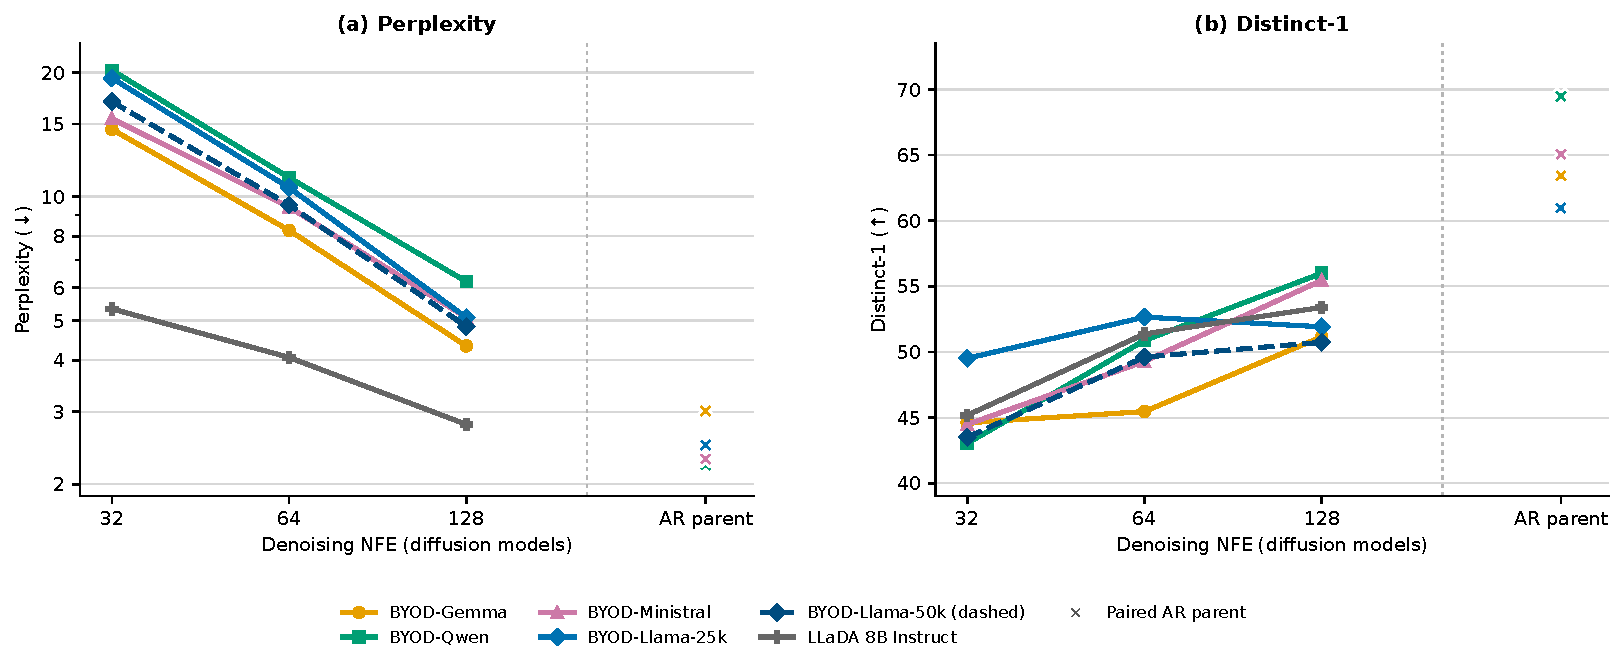
\includegraphics[width=\textwidth]{figures/open_generation_budget.pdf}
\caption{Fluency metrics for different models with different NFE budgets. Lines connect each diffusion model's results at 32, 64, and 128 NFE; crosses to the right show the corresponding AR-parent reference. Perplexity is shown on a logarithmic axis.}
\label{fig:open-generation-budget}
\end{figure*}

Figure~\ref{fig:open-generation-budget} shows that perplexity and Distinct-1 generally improve with additional NFE. At 64 NFE, converted models have 2.7--5.0 times their AR parents' perplexity and generally lower Distinct-$n$ (Appendix~\ref{app:open-generation-results}). BYOD-Gemma's perplexity is 14.56 at 32 NFE and 4.33 at 128 NFE, compared with 3.01 for its AR parent under standard sequential generation. The AR result provides a quality reference; these decoding regimes do not establish equal compute or latency. For simplicity, we discuss Distinct-1 in the main text; appendix results for Distinct-1/2/3 show the same broad pattern. LLaDA also has lower perplexity than every BYOD model. Representative samples are provided in Appendix~\ref{app:demo-trajectories} to illustrate iterative refinement under different remasking strategies and NFE budgets.

\subsection{Further training}

The expanded benchmark results show no clear average accuracy gain from further training (Table~\ref{tab:accuracy}). Figure~\ref{fig:llama-training-diagnostics} shows that validation loss decreases almost monotonically and begins to plateau toward the end of 50,000 training updates. Perplexity also decreases across all NFE budgets, but with larger fluctuations between checkpoints. Distinct-1 changes comparatively little and remains broadly stable. BYOD-Llama perplexity remains well above LLaDA, whose perplexity is in turn above the Llama AR baseline. In contrast, BYOD-Llama and LLaDA have similar Distinct-1 scores, while the AR baseline remains higher.

\begin{figure*}[t]
\centering
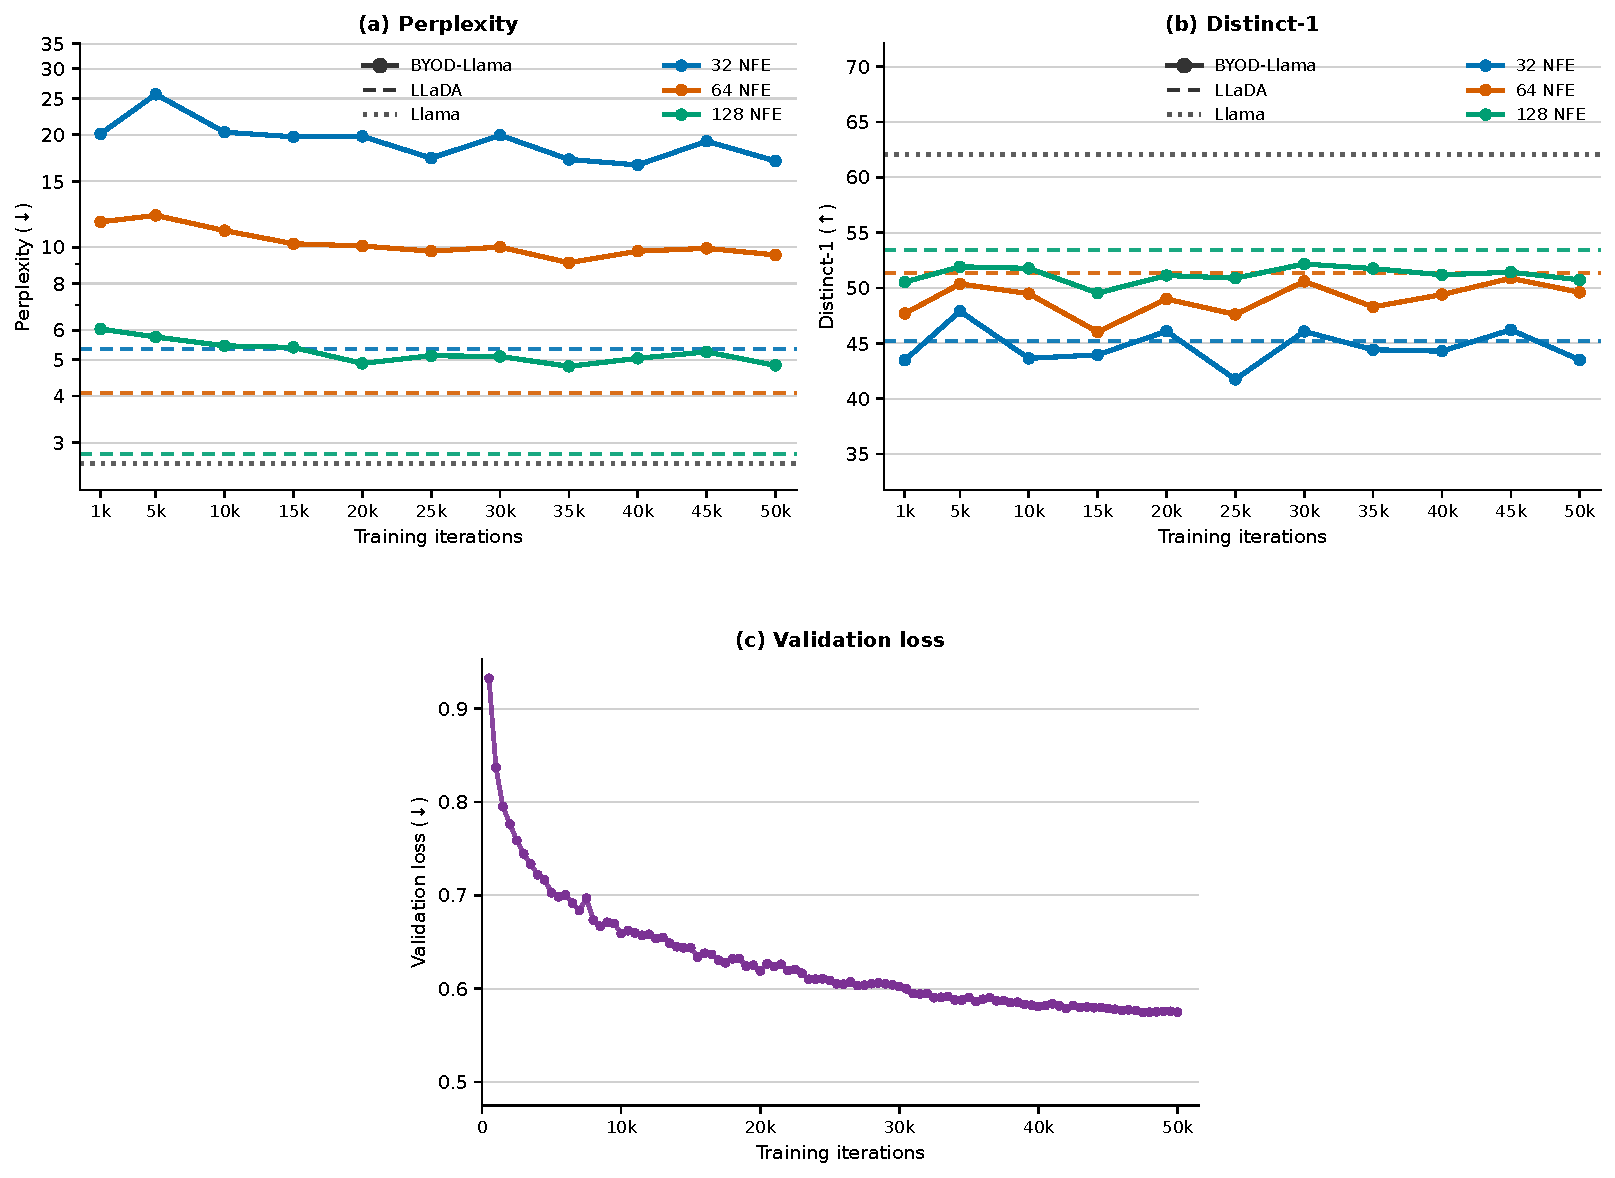
\includegraphics[width=\textwidth]{figures/llama_training_diagnostics.pdf}
\caption{BYOD-Llama-50k training diagnostics. (a) Token-weighted Phi-4 perplexity for 128-token generations, shown on a logarithmic y-axis. (b) Mean sliding model-token Distinct-1 for the same generations, reported as a percentage. Color-matched dashed lines are fixed LLaDA references; the dotted gray line is the unchanged Llama AR parent. (c) Validation loss.}
\label{fig:llama-training-diagnostics}
\end{figure*}

\subsection{Bidirectional attention test}
\label{sec:bidirectional-infilling}

Adding the later clue changed the greedy prediction on 100\% of test items for every converted model and LLaDA, confirming that all models use right-context information. BYOD-Gemma, BYOD-Ministral, and LLaDA copied the visible target exactly in 100\% of cases; BYOD-Llama-25k, BYOD-Llama-50k, and BYOD-Qwen reached 90\%, 70\%, and 20\%, respectively. Without the clue, exact-match accuracy was 0\% for every model. Appendix~\ref{app:bidirectional-infilling} reports the complete results and protocol.

\section{Discussion}

The central result is that high-rank attention-only LoRA can convert four AR models into DLMs in a few hours on a single GPU. All converted models have lower mean task accuracy than their AR parents. BYOD-Gemma's mathematics and coding scores fall in a similar range to LLaDA's, with mixed task-level differences, despite its much smaller additional training budget. This supports LoRA adaptation as a practical route to useful diffusion models, while the perplexity gap shows that task-score proximity does not establish overall equivalence. The comparison does not establish superiority over full-parameter training: the models differ in size and training history, and we did not run a matched full-fine-tuning control. The strongest observed conversion was also selected from several configurations, without selection-adjusted uncertainty. Several aspects of these findings warrant closer examination, and are discussed below.

Conversion quality varies by backbone: BYOD-Gemma has the highest BYOD mean despite Qwen having the strongest AR parent, so parent capability alone does not determine conversion quality. Gemma's larger model and adapter budget may contribute, but cannot be separated here. The largest benchmark deficits relative to the AR parents occur in mathematics and code. Parser checks reveal much more frequent syntax errors in the converted models; AR errors are rare but not entirely absent (Appendix~\ref{app:code-errors}). This is consistent with prior work showing that parallel token prediction in DLMs can produce syntactic inconsistencies \citep{hersche2026codila}.

Although generation under full NFE budgets generally produces coherent sentences, perplexity and Distinct-1/2/3 still trail both the AR parents and LLaDA, especially when NFE is below output length. This is also noticeable qualitatively when using the models through the demo interface. Extending Llama training from 25,000 to 50,000 updates gives mixed task-level changes and no clear average accuracy benefit. While validation loss still decreases almost monotonically during the longer run, these downstream results suggest that longer training alone may be insufficient; useful ablations would include larger effective batches, alternative denoising targets, and adapters in key/output projections, MLPs, or normalization layers.

Even though we used perplexity and Distinct-1/2/3 as proxies for fluency, they are not sufficient to reliably predict human preference. For example, an external AR perplexity scoring model can favor repetitive high-probability text. While Distinct-$n$ captures this repetition, these metrics still do not measure factuality, grammar, or coherence \citep{gong2025diffullama,turok2026duel}. We therefore combine perplexity, Distinct-1/2/3, task accuracy, and demos for qualitative inspection of generated samples, rather than treating any one metric as definitive.

In the bidirectionality test, every converted model changed its prediction on every item when the later clue was added, demonstrating bidirectional attention across all four families. Some models did not always copy the token correctly, indicating a failure to use the clue rather than an absence of information flow. The public demos enable quick experimentation with NFE, output length, remasking, and blockwise generation, while exposing grammaticality, coherence, and denoising errors that aggregate metrics cannot capture.

LoRA keeps all original parameters frozen during conversion, preventing their direct overwriting and potentially reducing catastrophic forgetting \citep{luo2023catastrophic}. We chose \(r=1024\) to balance denoising quality with single-GPU training: the original implementation accommodated a per-device batch of 16 on an 80GB A100, or 8 on a 40GB A100. The separate rank ablation shows that larger ranks lower validation loss, with diminishing loss reductions per added adapter parameter (Appendix~\ref{app:rank-ablation}). Rank 2048 still gives lower loss, but doubles the adapter parameters and takes longer per update. This single-parent, single-seed study does not establish an optimal rank for downstream accuracy or other backbones. Earlier exploratory trials informed our target-module and learning-rate choices; their joint sensitivity remains outside the present ablation.

It should be noted that the high-rank adapters can subsequently be merged into the base projections. This removes their temporary parameter and inference overhead while restoring the original model size with broadly similar behavior, as shown by our experiments (Appendix~\ref{app:merge}). Future work could study whether merged models could subsequently initialize partial or full diffusion fine-tuning; establishing diffusion generation before exposing the original weights to optimization may make these updates less disruptive.

Finally, although one conversion takes only a few hours, development and evaluation across models, configurations, ablations, and validation runs required hundreds of GPU-hours. Nevertheless, BYOD reuses an AR checkpoint and processes orders of magnitude fewer token positions than the full-model systems in Table~\ref{tab:compute}, enabling repeatable cross-architecture experiments without repeated pretraining. This does not erase the original pretraining cost or establish a proportional reduction in emissions.

\section{Limitations}
The main limitation is that efficient conversion does not yet produce efficient generation, as output quality is not yet on par with the AR parents or LLaDA, especially when NFE is below output length. We also measure inference budget in network evaluations rather than wall-clock latency. Fewer sequential evaluations do not guarantee a speedup because each diffusion step processes the full answer block. Our efficiency claim therefore concerns training the conversion, not measured inference acceleration.

The cross-backbone comparison is not a controlled architecture study. The parents differ in size, tokenizer, pretraining, alignment, and attention design. Fixing LoRA rank also gives each backbone a different absolute adapter budget. Gemma's leading result therefore cannot be attributed separately to architecture, parent quality, model size, or trainable parameter count.

The benchmark intervals describe item variation within nine fixed tasks, not variation across training seeds or task families; they do not correct systematic subset-selection effects or multiple model comparisons. In particular, the nominal Gemma--LLaDA interval is not adjusted for selecting Gemma as the strongest observed conversion. Their different sizes and training histories also prevent attributing the comparison to LoRA versus full-parameter training. The expanded scores include uniform MATH rescoring and a fresh BYOD-Gemma cohort, so changes from the submitted scores cannot all be attributed to larger sample counts (Appendix~\ref{app:benchmark-uncertainty}).

Finally, the automatic generation metrics cover only part of text quality. Phi-4 perplexity reflects the preferences of an external AR model, while Distinct-$n$ detects local repetition but not factuality, grammar, or coherence. Published results from other DLMs use different protocols; only LLaDA was rerun in our harness. We also did not measure energy use or carbon intensity directly, so claims on cost or resource efficiency should only be taken as indicative of relative scale rather than a measured (environmental) footprint.

\section{Conclusion}

\method{} converts instruction-tuned AR checkpoints across four families into bidirectional masked generators in a few hours on one Google Colab GPU while retaining substantial parent-model knowledge. Fluency and diversity nevertheless trail the AR parents and LLaDA, especially when NFE is below output length. A promising next step is partial or full diffusion fine-tuning initialized from the merged model, testing whether quality can improve without eroding retained capabilities. BYOD thereby enables rapid, controlled diffusion experiments across established model families with minimal compute infrastructure.


\section*{Reproducibility Statement}

Training and evaluation code and model weights will be released upon acceptance. Anonymous full-precision ZeroGPU demos are provided for all four conversions. The main text specifies the objective, trainable modules, data volume, optimization, generation, benchmarks, and scoring; the archival release will include resolved configurations, parameter audits, checkpoint identifiers, loss logs, generated samples, and benchmark manifests.

\section*{Ethics Statement}

This study uses existing language models and public benchmark or instruction datasets and does not involve human subjects. Converted models inherit factual errors, biases, unsafe behaviors, licensing constraints, and memorization risks from their parent checkpoints and training data. We report aggregate task performance rather than claiming safety or deployment readiness; release artifacts should preserve upstream licenses and document the data provenance and intended research use.

\section*{AI Use Statement}

Generative AI tools were used to assist software development and debugging, creation of analysis scripts, literature discovery and summarization, creation of the open-ended question dataset, and drafting and editing this manuscript. The authors manually reviewed AI-assisted code and prose, and verified literature claims and citations against primary sources. No benchmark value was entered solely from an unsupported model response. The authors take responsibility for the final content, claims, code, and artifacts.

\bibliography{iclr2027_conference}
\bibliographystyle{iclr2027_conference}

\appendix
\section{Cost and operational-emissions estimation}
\label{app:cost}

Table~\ref{tab:compute} compares the cost of training a model that produces diffusion behavior. It should thus be taken into account that some of these models build on an AR parent, whereas others are trained from scratch. It also excludes exploratory runs, failed jobs, dataset construction, evaluation, storage, and inference. The estimates must therefore not be interpreted as total project or lifecycle footprints.

For BYOD we use the observed 3.2 GPU-hours for the conversion of a Llama 3.1 8B model for diffusive generation. For a prior work that reports GPU-hours, we retain that value. Where a paper reports model size but not time, we approximate training compute as $C\approx6ND$ FLOPs \citep{hoffmann2022chinchilla}, where $C$ is total training compute, $N$ is the number of model parameters, and $D$ is the number of processed training-token positions. We then calculate
\begin{equation}
G_{\mathrm{est}}=\frac{6ND}{0.40\,(989\times10^{12})\,3600},
\end{equation}
where $G_{\mathrm{est}}$ is aggregate estimated GPU-hours, 0.40 is the assumed model FLOPs utilization (MFU), $989\times10^{12}$ is the NVIDIA H100's dense BF16 Tensor Core throughput in FLOP/s \citep{nvidiaH100}, and 3600 converts seconds to hours. The 40\% MFU assumption is consistent with the 39.0--45.0\% BF16 MFUs reported by FP8-LM for GPT-style 7B, 13B, and 175B training on H100 GPUs \citep{peng2023fp8lm}. Actual utilization varies considerably with architecture, sequence length, parallelization, communication, activation recomputation, and implementation efficiency. The assumption is therefore a standardized order-of-magnitude convention rather than a reconstruction of any authors' cluster. It yields the daggered values in Table~\ref{tab:compute}. The Dream and iLLaDA estimates cover their main 580B- and 12T-token stages but omit the smaller instruction-tuning additions, so they are lower bounds.

Table~\ref{tab:compute-calibration} calibrates the same calculation against studies that report both a usable token count and elapsed accelerator-hours \citep{nie2025llada,wu2025fastdllmv2}. For LLaDA, it predicts approximately 77,519 GPU-hours, compared with 130,000 reported H800 GPU-hours, corresponding to an implied utilization of 23.9\%. Thus 40\% can be optimistic about achieved utilization and correspondingly conservative with respect to estimated accelerator-hours, rental cost, and emissions. Fast-dLLM v2 displays a still larger gap. Its specialized training concatenates clean and noised views and uses a nonstandard attention pattern, illustrating that an ``implied MFU'' from $6ND$ is a calibration diagnostic, not a measured hardware-utilization statistic.

\begin{table}[h]
\caption{Calibration of the $6ND$ estimator against reported accelerator-hours. Predictions use 40\% MFU and the stated accelerator's dense-BF16 peak (989 TFLOP/s H100-class proxy for H800; 312 TFLOP/s for A100) \citep{nvidiaH100,nvidiaA100}. ``Implied MFU'' is the utilization that would reconcile $6ND$ with reported time; it is not a measured MFU.}
\label{tab:compute-calibration}
\centering
\small
\begin{tabular}{lrrrrr}
\toprule
System & Parameters & Tokens & Pred. GPU-h & Reported GPU-h & Implied MFU \\
\midrule
LLaDA & 8B & 2.30T & 77,519 & 130,000 & 23.9\% \\
Fast-dLLM v2 & 7B & 1.31B & 123 & 768 & 6.4\% \\
\bottomrule
\end{tabular}
\end{table}

We convert BYOD time to a rental-equivalent cost using the September 2026 AWS US-East on-demand price of \$3.36 per hour for a one-GPU \texttt{g7e.2xlarge}, obtained from the AWS Price List. AWS specifies that this instance contains the same 96-GB NVIDIA RTX PRO 6000 Blackwell Server Edition GPU used in our Colab run \citep{awsPriceListG7e2026,awsG7e2026}. For other systems we use one consistent current major-cloud proxy: \$5.191 per accelerator-hour for an AWS \texttt{p5.4xlarge} H100 Capacity Block in US East \citep{awsCapacity2026}. Thus these figures answer ``what would the stated or estimated accelerator-hours cost at a public contemporary rate?'', not what the original authors paid. They exclude storage, egress, idle reservation time, taxes, and discounts.

Operational emissions are estimated as energy use multiplied by the data center's power usage effectiveness (PUE) and the grid carbon intensity \citep{lannelongue2021green,patterson2021carbon}:
\begin{equation}
\widehat{E}_{\mathrm{CO_2e}}=G\,P_{\mathrm{GPU}}\,\mathrm{PUE}\,I_{\mathrm{grid}}.
\end{equation}
Here $\widehat{E}_{\mathrm{CO_2e}}$ is estimated operational emissions in kg CO$_2$e, $G$ is aggregate GPU-hours, $P_{\mathrm{GPU}}$ is assumed per-GPU power draw in kW, PUE is the dimensionless data-center power usage effectiveness, and $I_{\mathrm{grid}}$ is grid carbon intensity in kg CO$_2$e/kWh. We use 0.60 kW for RTX PRO 6000 runs, matching NVIDIA's stated maximum board power \citep{nvidiaRTXPro6000}, and a 0.70-kW H100-class proxy for all other entries except the reported A100 run, for which we use 0.40 kW \citep{nvidiaH100,nvidiaA100}. We assume PUE 1.09, Google's reported fleet-wide value \citep{googlePUE2025}, and the IEA's 2024 global-average generation intensity of 0.445 kg CO$_2$e/kWh \citep{ieaElectricity2025}. For example, one BYOD stage gives $3.2\times0.60\times1.09\times0.445=0.93$ kg CO$_2$e. These are location-independent GPU-only operating scenarios: they assume full rated GPU power, omit host CPU/memory/network energy and embodied hardware emissions, and do not account for renewable-energy procurement. Direct power telemetry and the datacenter's time- and location-specific marginal carbon intensity would be required for a measured footprint.

\section{Comparison with LAD}
\label{app:lad-comparison}

\method{} inherits the use of attention-projection LoRA and bidirectional attention from LAD \citep{kuiper2025lad}. The question tested here is whether a shared mask-only conversion recipe transfers across Gemma, Llama, Qwen and Ministral. LAD evaluated Llama 3.2 1B/3B and Llama 3.1 8B, with two ranks per size. Its corruption combines masking with swaps, duplications and span shifts, and its generation procedure can revise visible tokens as well as masked positions. This differs from the mask-only MDLM setup studied here.

\paragraph{Implementation and training settings.} Both methods target the query and value projections with LoRA, use bidirectional attention, set $\alpha=r$, and use zero adapter dropout. LAD varies rank from 128 to 2048 across its model sizes; \method{} fixes rank 1024 across all four families. LAD trains for 100,000 updates at batch size 8, whereas our primary conversions use 25,000 updates at batch size 16. Both use a maximum training sequence length of 256, giving approximately 204.8M token positions for LAD and at most 102.4M for each primary BYOD conversion. These are different published training setups, rather than matched-budget experiments.

\begin{table}[ht]
\caption{Benchmark accuracy (\%) under separate protocols. LAD values are transcribed from Table~2 of \citet{kuiper2025lad}, using 100 examples per task. BYOD-Llama-25k uses the expanded 250-example evaluation reported in Table~\ref{tab:accuracy}. A dash means the task was not evaluated for BYOD. No scores in this table come from a new matched LAD experiment.}
\label{tab:lad-comparison}
\centering
\small
\begin{tabular}{lrrr}
\toprule
Task & LAD 8B, $r=1024$ & LAD 8B, $r=2048$ & BYOD-Llama-25k \\
\midrule
ARC-Easy & 93.0 & 93.0 & \na \\
ARC-Challenge & 79.0 & 80.0 & 82.8 \\
HellaSwag & 80.0 & 76.0 & 72.8 \\
MMLU & 54.0 & 53.0 & 61.2 \\
GSM8K & 44.0 & 45.0 & 64.8 \\
\bottomrule
\end{tabular}
\end{table}

Both 8B conversions start from Llama 3.1 8B Instruct, but their training and evaluation settings differ. LAD judges generated answers with GPT-4o and uses semi-autoregressive generation on GSM8K, whereas our harness uses task-specific answer extraction and scoring. The evaluated question sets, generation settings and training budgets are also not matched. Table~\ref{tab:lad-comparison} therefore provides context rather than a ranking of the methods or an estimate of the effect of removing structured corruption. A common-data, common-budget comparison would be needed to isolate that effect.

\section{LoRA-rank ablation}
\label{app:rank-ablation}

We run a separate validation-loss experiment on Llama 3.1 8B Instruct at ranks 128, 512, 1024 and 2048. All runs use Q/V adapters, $\alpha=r$, zero adapter dropout, frozen backbone parameters, the same data order and seed (42), batch size 16, sequence length 256, and a learning rate of $10^{-5}$ with cosine decay and 100 warmup updates. Each run completes 25,000 updates. The validation objective is $0.9\,\mathcal{L}_{\mathrm{answer}}+0.1\,\mathcal{L}_{\mathrm{padding}}$, with each term normalized separately. We evaluate the same 200 validation examples with fixed corruptions every 250 updates. These runs do not replace the original benchmarked BYOD-Llama model.

\begin{figure}[ht]
\centering
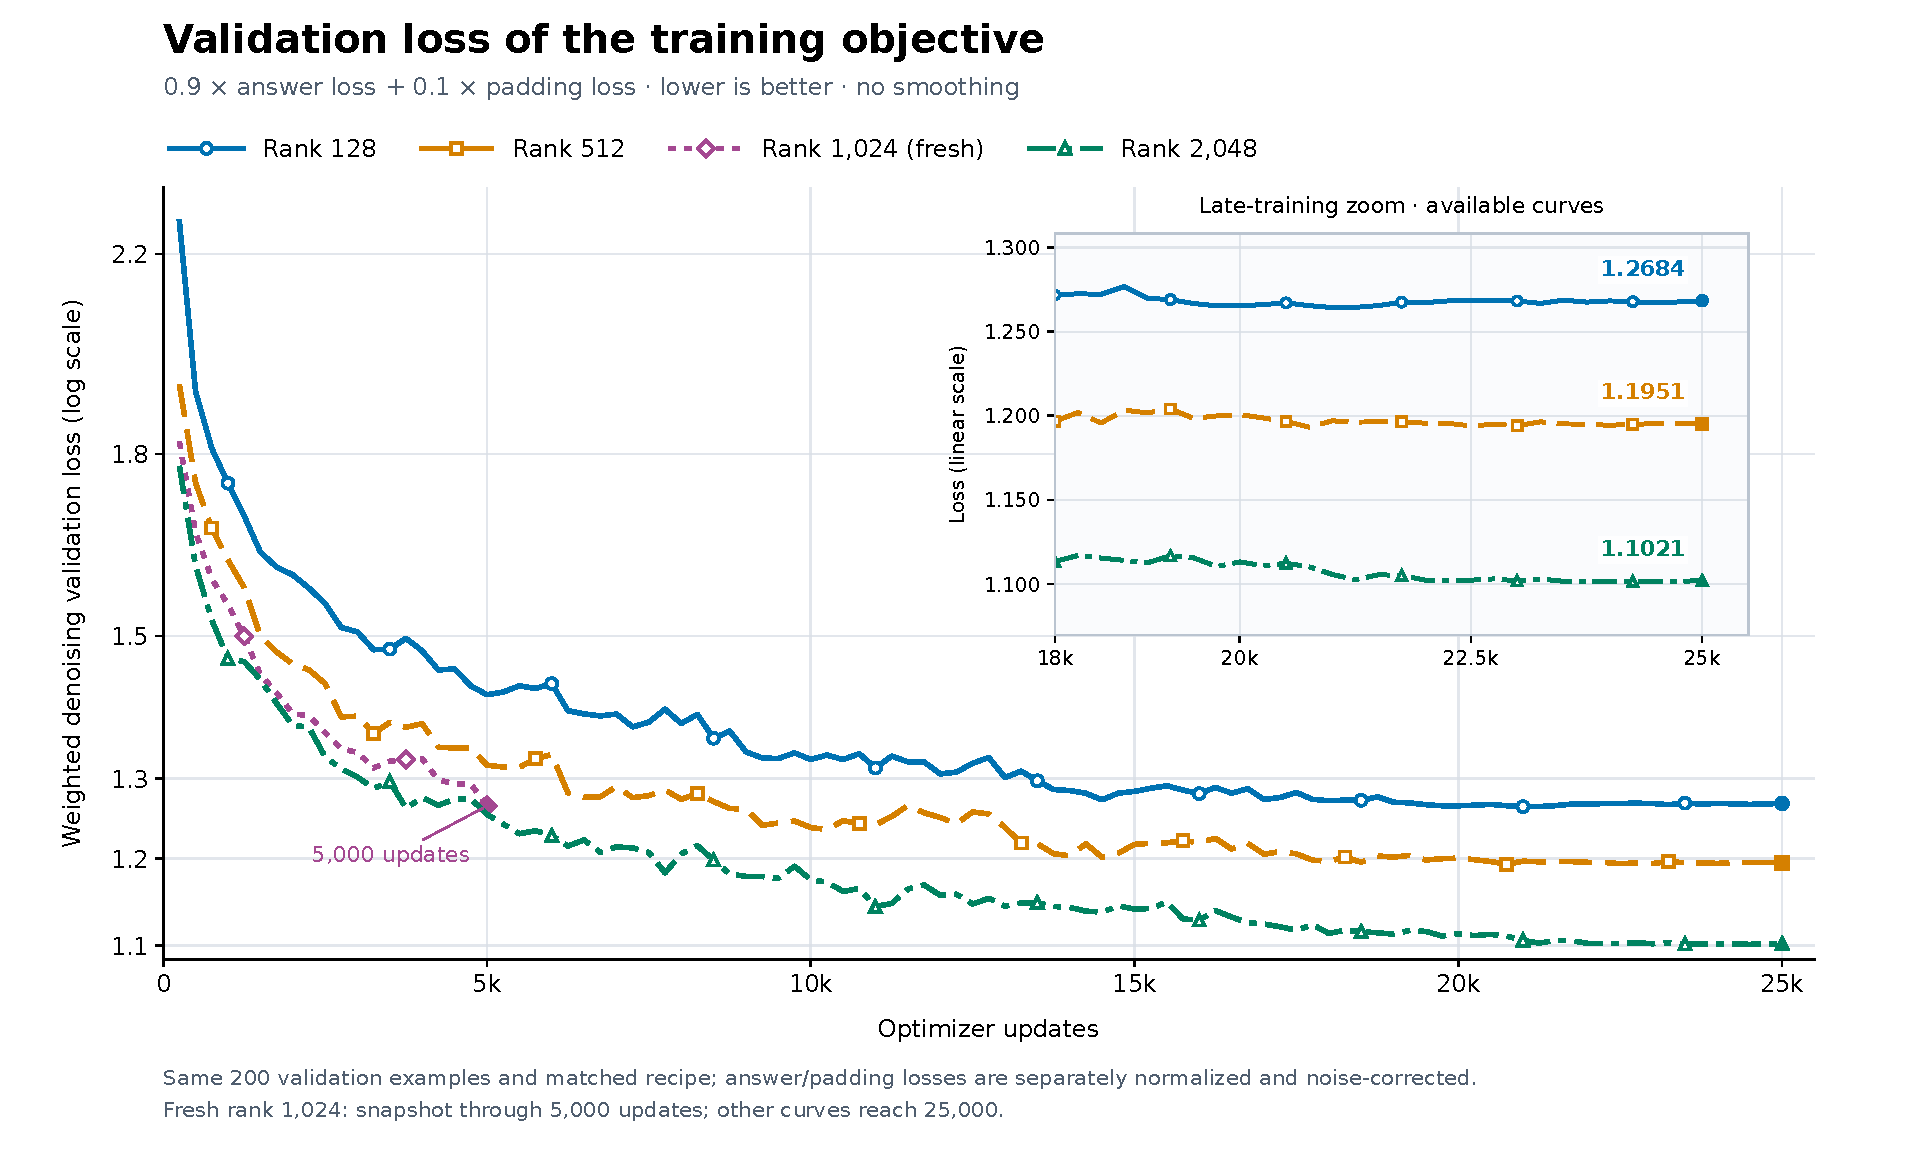
\includegraphics[width=\textwidth]{figures/rank_validation_training_objective.pdf}
\caption{Validation loss for the separate rank ablation. The vertical axis shows the actual 90/10-weighted training objective on a logarithmic scale; the inset expands late training. Blue circles, orange squares, purple diamonds and green triangles denote ranks 128, 512, 1024 and 2048, respectively. All four ranks reach 25,000 updates. The historical rank-1024 training curve is excluded.}
\label{fig:rank-ablation}
\end{figure}

\begin{table}[ht]
\caption{Rank trade-off at 25,000 matched updates. Update times are medians of clean 100-update logging intervals, excluding validation, checkpoint saving and restart-clock resets; they are not end-to-end training durations.}
\label{tab:rank-tradeoff}
\centering
\small
\begin{tabular}{rrrr}
\toprule
Rank & Adapter parameters (M) & Validation loss at 25k & Seconds/update \\
\midrule
128 & 54.5 & 1.2684 & 0.374 \\
512 & 218.1 & 1.1951 & 0.386 \\
1024 & 436.2 & 1.1525 & 0.403 \\
2048 & 872.4 & 1.1021 & 0.434 \\
\bottomrule
\end{tabular}
\end{table}

Rank 1024 was chosen to balance validation quality with single-A100 training. In the original implementation, this accommodated per-device batch size 16 on an 80GB A100 or batch size 8 on a 40GB A100. These configurations describe the original implementation; the controlled rank study uses RTX PRO 6000 GPUs. Memory requirements depend on implementation and training settings.

At 25,000 matched updates, increasing rank from 512 to 1024 reduces validation loss by 0.0427; increasing it from 1024 to 2048 reduces loss by 0.0504. The latter increase adds twice as many rank units and adapter parameters: 436.2M rather than 218.1M additional parameters. The loss reduction per added parameter is therefore about 41\% smaller for the latter increase. This is a diminishing return per added parameter, rather than necessarily a smaller absolute loss reduction.

Rank 2048 takes about 7.6\% longer per update than rank 1024 and doubles its adapter parameter count. The runs use the same RTX PRO 6000 GPU type, with rank 1024 using separate allocations. At fixed precision and optimizer, adapter parameters, gradients and optimizer state grow with rank. This is not a measured comparison of peak GPU memory across ranks.

These results support rank 1024 as a practical quality/resource trade-off under the original single-GPU constraint; rank 2048 still gives lower validation loss. They do not establish a globally optimal rank or downstream benchmark gains: this is a validation-only experiment on one parent and one seed. Earlier exploratory tests of other attention-projection targets, MLP adapters and learning rates informed our configuration, but were not retained as a systematic controlled sweep. A full search over these interacting choices was outside this study's scope.

Label alignment and the 0.9/0.1 answer/padding loss weights remain fixed throughout this rank study. Unshifted labels implement the same-position reconstruction target in Equation~\ref{eq:region-loss}; we have not independently ablated this alignment. Earlier exploratory loss-weight trials informed the configuration, but do not establish optimal weights or replace a controlled sensitivity study.


\section{Benchmark coverage and uncertainty}
\label{app:benchmark-uncertainty}

\paragraph{Coverage.} All ten configurations use the same questions within each task. Table~\ref{tab:benchmark-coverage} lists the full available evaluation splits and our evaluated counts. The completed selection contains 21,640 model--question outcomes, compared with 11,070 recovered historical outcomes: a net increase of 10,570 selected outcomes. This increase excludes replacement generations and diagnostic runs. Eight tasks now have 250 questions per configuration, doubling the usual historical count of 125; HumanEval uses all 164 available questions. Sanitized MBPP has 257 test questions, of which we evaluate 250.

\begin{table}[ht]
\caption{Available evaluation-set sizes and actual questions evaluated per configuration. The same selection is used for every model. The released GPQA split is named \texttt{train}, but is used only for evaluation here. HellaSwag uses labeled validation data.}
\label{tab:benchmark-coverage}
\centering
\small
\begin{tabular}{llrr}
\toprule
Task & Evaluation split & Available & Evaluated/model \\
\midrule
ARC-Challenge & Test & 1,172 & 250 \\
GPQA-Main & \texttt{gpqa\_main/train} & 448 & 250 \\
HellaSwag & Validation & 10,042 & 250 \\
MMLU & \texttt{all/test} & 14,042 & 250 \\
MMLU-Pro & Test & 12,032 & 250 \\
GSM8K & \texttt{main/test} & 1,319 & 250 \\
MATH-500 & Test & 500 & 250 \\
HumanEval & Test & 164 & 164 \\
MBPP sanitized & \texttt{sanitized/test} & 257 & 250 \\
\midrule
Total per configuration & & & 2,164 \\
\bottomrule
\end{tabular}
\end{table}

\paragraph{Individual task intervals.} Tables~\ref{tab:benchmark-intervals-1}--\ref{tab:benchmark-intervals-3} give the complete common-harness results with nominal 95\% Wilson score intervals. For $k$ correct answers out of $n$, $\hat p=k/n$ and $z=1.959964$, the endpoints are
\begin{equation}
\frac{\hat p+z^2/(2n)\;\pm\;z\sqrt{\hat p(1-\hat p)/n+z^2/(4n^2)}}{1+z^2/n}.
\end{equation}
These are computed from integer counts, before rounding. At $n=250$, the worst-case half-width is about 6.15 percentage points; doubling the evaluation does not produce per-task precision of $\pm1$--2 points. Evaluating all HumanEval questions removes subsampling uncertainty for that fixed test set under the stated decoding protocol. Its Wilson interval instead concerns an interpretation of those problems as observations from a broader population of items.

\paragraph{Averages and paired differences.} We compute $A=\frac{1}{9}\sum_{t=1}^{9}\hat p_t$, giving every task equal weight despite the smaller HumanEval set. For each of 20,000 bootstrap replicates, questions are resampled with replacement separately within each task, with the original task sample sizes retained. The 2.5th and 97.5th percentiles give the mean's interval (seed 20261116). For a model difference, both models use the same resampled question IDs within a task, retaining their pairing (20,000 replicates, seed 20261115). We do not subtract the endpoints of the two separate model intervals. All intervals are nominal 95\% intervals without a multiple-comparison adjustment. They describe empirical item variation within these nine fixed tasks, not variation across training seeds or uncertainty over new task families, and do not correct systematic subset-selection effects.

The paired BYOD-Gemma minus LLaDA difference is +2.88 points [0.74, 4.98]; BYOD-Gemma minus Gemma AR is $-10.30$ points [$-12.33$, $-8.31$]; and BYOD-Llama-50k minus BYOD-Llama-25k is $-0.14$ points [$-1.81$, 1.49]. These are descriptive, nominal intervals under the reported question sets and method-specific generation settings. They do not provide simultaneous 95\% coverage across the five BYOD configurations, including the longer Llama run, or adjust for selecting Gemma as the strongest conversion. Its 9B parent also differs from 8B LLaDA in size and training history. We therefore make no superiority claim from this comparison. A matched full-parameter adaptation control would be needed to compare the conversion methods themselves. Published external scores have no intervals computed here because their per-question outputs are unavailable to this analysis.

\paragraph{Provenance and corrections.} Compatible historical generations were retained after checking model assets, prompts, targets and settings. All BYOD-Gemma tasks were regenerated as a complete cohort after historical replay differences, rather than selecting improved answers. New Qwen AR answers generated with a faulty eager-attention path were replaced consistently using SDPA, while verified historical answers were retained. MATH was rescored uniformly with final-answer normalization and pinned symbolic verification, including numeric presentation and percentage-unit cases. Consequently, changes from the submitted values combine sample expansion, scoring corrections and these generation replacements; they are not solely a sample-size effect. Raw historical and replacement answers remain separate in the audit records.

% Generated from integer counts; 95% Wilson intervals, percentages.
\begin{table}[ht]
\caption{Complete benchmark accuracy and nominal 95\% Wilson intervals (\%), panel 1 of 3. HumanEval uses all 164 items; every other task uses 250. The same items are used for all models.}
\label{tab:benchmark-intervals-1}
\centering
\small
\begin{tabular}{lrrr}
\toprule
Model & ARC-C & GPQA-Main & HellaSwag \\
\midrule
BYOD-Gemma & 90.0 [85.7, 93.1] & 30.8 [25.4, 36.8] & 78.8 [73.3, 83.4] \\
Gemma AR & 88.8 [84.3, 92.1] & 29.6 [24.3, 35.5] & 70.4 [64.5, 75.7] \\
BYOD-Qwen & 84.0 [78.9, 88.0] & 31.2 [25.8, 37.2] & 73.6 [67.8, 78.7] \\
Qwen AR & 90.0 [85.7, 93.1] & 33.6 [28.0, 39.7] & 74.4 [68.6, 79.4] \\
BYOD-Ministral & 82.0 [76.8, 86.3] & 30.8 [25.4, 36.8] & 76.8 [71.2, 81.6] \\
Ministral AR & 72.0 [66.1, 77.2] & 32.4 [26.9, 38.4] & 72.4 [66.6, 77.6] \\
BYOD-Llama-25k & 82.8 [77.6, 87.0] & 27.6 [22.4, 33.4] & 72.8 [67.0, 77.9] \\
BYOD-Llama-50k & 81.6 [76.3, 85.9] & 28.0 [22.8, 33.9] & 77.2 [71.6, 82.0] \\
Llama AR & 78.0 [72.5, 82.7] & 27.2 [22.1, 33.0] & 58.8 [52.6, 64.7] \\
LLaDA & 86.8 [82.0, 90.4] & 31.2 [25.8, 37.2] & 69.6 [63.6, 75.0] \\
\bottomrule
\end{tabular}
\end{table}

\begin{table}[ht]
\caption{Complete benchmark accuracy and nominal 95\% Wilson intervals (\%), panel 2 of 3. HumanEval uses all 164 items; every other task uses 250. The same items are used for all models.}
\label{tab:benchmark-intervals-2}
\centering
\small
\begin{tabular}{lrrr}
\toprule
Model & MMLU & MMLU-Pro & GSM8K \\
\midrule
BYOD-Gemma & 66.4 [60.3, 72.0] & 39.2 [33.4, 45.4] & 68.8 [62.8, 74.2] \\
Gemma AR & 65.6 [59.5, 71.2] & 44.4 [38.4, 50.6] & 88.4 [83.8, 91.8] \\
BYOD-Qwen & 60.4 [54.2, 66.3] & 32.0 [26.5, 38.0] & 59.2 [53.0, 65.1] \\
Qwen AR & 69.2 [63.2, 74.6] & 46.4 [40.3, 52.6] & 92.4 [88.4, 95.1] \\
BYOD-Ministral & 58.4 [52.2, 64.3] & 32.8 [27.3, 38.8] & 66.4 [60.3, 72.0] \\
Ministral AR & 54.8 [48.6, 60.9] & 35.6 [29.9, 41.7] & 90.0 [85.7, 93.1] \\
BYOD-Llama-25k & 61.2 [55.0, 67.0] & 33.6 [28.0, 39.7] & 64.8 [58.7, 70.5] \\
BYOD-Llama-50k & 60.0 [53.8, 65.9] & 31.6 [26.2, 37.6] & 60.8 [54.6, 66.6] \\
Llama AR & 56.0 [49.8, 62.0] & 43.2 [37.2, 49.4] & 85.2 [80.3, 89.1] \\
LLaDA & 58.4 [52.2, 64.3] & 36.8 [31.1, 42.9] & 59.6 [53.4, 65.5] \\
\bottomrule
\end{tabular}
\end{table}

\begin{table}[ht]
\caption{Complete benchmark accuracy and nominal 95\% Wilson intervals (\%), panel 3 of 3. HumanEval uses all 164 items; every other task uses 250. The same items are used for all models.}
\label{tab:benchmark-intervals-3}
\centering
\small
\begin{tabular}{lrrr}
\toprule
Model & MATH-500 & HumanEval & MBPP sanitized \\
\midrule
BYOD-Gemma & 24.4 [19.5, 30.1] & 29.9 [23.4, 37.3] & 43.6 [37.6, 49.8] \\
Gemma AR & 52.0 [45.8, 58.1] & 59.8 [52.1, 67.0] & 65.6 [59.5, 71.2] \\
BYOD-Qwen & 30.4 [25.0, 36.4] & 23.8 [17.9, 30.8] & 40.0 [34.1, 46.2] \\
Qwen AR & 73.6 [67.8, 78.7] & 81.1 [74.4, 86.4] & 75.2 [69.5, 80.1] \\
BYOD-Ministral & 20.4 [15.9, 25.8] & 29.3 [22.8, 36.6] & 40.0 [34.1, 46.2] \\
Ministral AR & 56.0 [49.8, 62.0] & 82.3 [75.8, 87.4] & 68.8 [62.8, 74.2] \\
BYOD-Llama-25k & 22.8 [18.0, 28.4] & 25.0 [19.0, 32.1] & 40.8 [34.9, 47.0] \\
BYOD-Llama-50k & 24.4 [19.5, 30.1] & 23.8 [17.9, 30.8] & 42.8 [36.8, 49.0] \\
Llama AR & 42.4 [36.4, 48.6] & 51.2 [43.6, 58.8] & 68.4 [62.4, 73.8] \\
LLaDA & 26.0 [21.0, 31.8] & 34.8 [27.9, 42.3] & 42.8 [36.8, 49.0] \\
\bottomrule
\end{tabular}
\end{table}


\section{Adapter-merging ablation}
\label{app:merge}

High-rank LoRA increases the parameter count only while the adapter remains separate. To test whether removing this overhead changes behavior, we evaluated the same BYOD-Llama-25k checkpoint with the adapter loaded and after its weights were folded into the base projections. Tables~\ref{tab:merge-open-generation} and~\ref{tab:merge-benchmarks} retain this separate historical comparison; it was not part of the expanded benchmark campaign.

\begin{table}[h]
\caption{Open-generation comparison of the adapter-loaded and merged Llama checkpoints. PPL is token-weighted; Distinct-$n$ is averaged over answers and reported as a percentage. Both use 128 generated tokens; D-1/2/3 use 32 NFE.}
\label{tab:merge-open-generation}
\centering
\scriptsize
\begin{tabular}{lrrrrrr}
\toprule
Representation & Parameters & PPL$_{32}\downarrow$ & PPL$_{128}\downarrow$ & D-1\%$\uparrow$ & D-2\%$\uparrow$ & D-3\%$\uparrow$ \\
\midrule
Adapter loaded & 8.466B & 19.381 & 5.081 & 49.5 & 78.8 & 89.9 \\
Merged standalone & 8.030B & 19.283 & 4.764 & 49.8 & 80.7 & 91.8 \\
\bottomrule
\end{tabular}
\end{table}


\begin{table}[h]
\caption{Separate historical paired evaluation before and after merging: accuracy (\%) on 125 questions per task under the original scoring protocol. The mean gives the nine tasks equal weight. These measurements were not expanded to the sample counts in Table~\ref{tab:accuracy}.}
\label{tab:merge-benchmarks}
\centering
\small
\begin{tabular}{lrr@{\qquad}lrr}
\toprule
Task & Adapter & Merged & Task & Adapter & Merged \\
\midrule
ARC-C      & 83.2 & 84.0 & MATH     & 25.6 & 24.8 \\
GPQA       & 29.6 & 30.4 & MBPP     & 43.2 & 41.6 \\
GSM8K      & 65.6 & 63.2 & MMLU     & 59.2 & 60.8 \\
HellaSwag  & 70.4 & 69.6 & MMLU-Pro & 30.4 & 30.4 \\
HumanEval  & 31.2 & 29.6 & \textbf{Mean} & \textbf{48.7} & \textbf{48.3} \\
\bottomrule
\end{tabular}
\end{table}

Merging is an algebraic reparameterization rather than an additional training stage: each base projection $W$ is replaced by $W+(\alpha/r)BA$, where $A$ and $B$ are the trained rank-$r$ LoRA matrices and $\alpha$ is their scaling parameter. Subject to floating-point rounding, evaluating the folded projection is equivalent to evaluating the base and LoRA branches separately. Open-generation metrics are slightly better after merging, while factual results vary modestly by task and the macro mean decreases by only 0.4 points. These reruns therefore support preservation of overall behavior, but are not precise enough to attribute task-level changes to merging; a logit-level deterministic parity test would isolate numerical merge error from generation and benchmark variance.

\section{Complete training configuration}
\label{app:training-settings}

Table~\ref{tab:training-settings} records the common resolved configuration of the four primary conversions, including optimization, precision, checkpointing, and validation. We use AdamW with BF16 master weights and Transformer Engine HYBRID FP8 execution. The exact one-million-example training mixture is \href{https://huggingface.co/datasets/Dovelove/BYOD-training-1m-256}{available anonymously}, with row-level source provenance and upstream licensing terms.

\begin{table*}[p]
\caption{Full common training configuration. Model-specific parent checkpoints, mask strings, and parameter counts appear in Table~\ref{tab:models}.}
\label{tab:training-settings}
\centering
\small
\resizebox{\textwidth}{!}{%
\begin{tabular}{ll@{\qquad}ll}
\toprule
Setting & Value & Setting & Value \\
\midrule
Training examples & 400,000 & Optimizer updates & 25,000 \\
Maximum sequence length & 256 & Dynamic padding multiple & 16 \\
Batch size & 16/16 & Gradient accumulation & 1 \\
Optimizer & AdamW & Peak learning rate & $10^{-5}$ \\
Schedule & cosine & Warmup & 100 updates \\
Weight decay & 0.01 & Maximum gradient norm & 0.5 \\
Training precision & FP8 HYBRID & Master/evaluation precision & BF16 \\
Gradient checkpointing & disabled & Selected-logit optimization & enabled \\
Corruption & IID mask-only & Noise time & $t\sim\mathcal{U}[0.001,1]$ \\
Mask-eligible region & answer + EOS padding & Loss region & corrupted answer + EOS padding \\
Answer/padding loss weights & 0.9/0.1 & Genuine answer EOS & included \\
LoRA targets & query/value projections & LoRA rank/scaling/dropout & 1024/1024/0 \\
Trainable normalization & disabled & Quantization & none \\
Validation & 200 examples/250 updates & Checkpoint interval & 1,000 updates \\
Data-loader workers & 4 & Prefetch factor & 4 \\
\bottomrule
\end{tabular}}
\end{table*}

BYOD-Llama-50k keeps the same batch size and objective but processes 800,000 examples over 50,000 updates, validates every 500 updates, and uses a linear learning-rate decay from $10^{-5}$ to $10^{-6}$. This run supplies the BYOD-Llama-50k results and the diagnostics in Figure~\ref{fig:llama-training-diagnostics}.

\section{Complete inference configuration}
\label{app:inference-settings}

Table~\ref{tab:diffusion-inference} separates task-specific diffusion budgets from the training configuration; benchmark sample counts are listed in Appendix~\ref{app:benchmark-uncertainty}. The fixed 100-question open-ended prompt set is \href{https://huggingface.co/datasets/Dovelove/BYOD-open-ended-questions}{available anonymously}. Unless overridden in the table, diffusion evaluation uses the official LLaDA-style fixed-transfer sampler, greedy predictions (temperature 0), low-confidence remasking, classifier-free guidance scale 0, one full-answer block, and no repetition penalty. Delayed EOS/EOT means that a predicted terminator is assigned the lowest retention confidence and may therefore be predicted but is accepted late. The open-ended diagnostic uses temperature 0.7.

\begin{table*}[h]
\caption{Task-specific masked-diffusion inference settings in the validation notebook. NFE is the number of denoising network evaluations.}
\label{tab:diffusion-inference}
\centering
\small
\resizebox{\textwidth}{!}{%
\begin{tabular}{lrrrrl}
\toprule
Task & Output tokens & NFE & Block length & Temperature & Terminator handling\\
\midrule
Open-ended & 128 & 128/64/32 & 128 & 0.7 & delayed retention\\
MMLU & 64 & 64 & 64 & 0 & ordinary\\
MMLU-Pro & 64 & 64 & 64 & 0 & delayed retention\\
HellaSwag & 64 & 64 & 64 & 0 & ordinary\\
ARC-Challenge & 64 & 64 & 64 & 0 & ordinary\\
GSM8K & 256 & 256 & 256 & 0 & delayed retention\\
MATH-500 & 256 & 256 & 256 & 0 & delayed retention\\
GPQA-Main & 128 & 128 & 128 & 0 & delayed retention\\
HumanEval & 256 & 256 & 256 & 0 & delayed retention\\
MBPP & 128 & 128 & 128 & 0 & delayed retention\\
Bidirectional attention & 1 masked word & 1 & \na & 0 & \na\\
\bottomrule
\end{tabular}
}
\end{table*}

\begin{table}[h]
\caption{Recovered historical maximum new tokens for greedy AR evaluation; longer AR limits were intentional.}
\label{tab:ar-inference}
\centering
\small
\begin{tabular}{lr@{\qquad}lr}
\toprule
Task & Tokens & Task & Tokens \\
\midrule
Open-ended & 128 & MMLU & 1,024 \\
MMLU-Pro & 2,048 & HellaSwag & 1,024 \\
ARC-Challenge & 1,024 & GSM8K & 1,024 \\
MATH-500 & 1,024 & GPQA-Main & 1,024 \\
HumanEval & 1,024 & MBPP & 1,024 \\
\bottomrule
\end{tabular}
\end{table}

Table~\ref{tab:ar-inference} reports the maximum-new-token budgets for greedy AR evaluation. These are listed separately because an AR token budget is not an NFE budget and should not be read as computational equivalence. On MMLU-Pro, the AR models often generated reasoning before the final answer, motivating a 2,048-token upper limit. They could stop earlier; this was not a fixed generated length. The diffusion models generally produced shorter, direct answers, motivating a shorter canvas to reduce evaluation cost. The recorded diffusion setting is 64 tokens and 64 NFE, correcting the submitted description of 128 tokens. This was a practical protocol choice, rather than a controlled demonstration that a longer diffusion budget would not improve accuracy.

The completed evaluation uses the same 250 questions per task across models, or all 164 HumanEval questions, while preserving these intentional method-specific output limits. Compatible historical answers are reused; the complete fresh BYOD-Gemma cohort and corrected Qwen AR additions are described in Appendix~\ref{app:benchmark-uncertainty}. Qwen AR uses SDPA attention after matched replay checks identified failures in the new eager-attention outputs. The common harness and shared questions enable paired comparisons, but do not equalize training exposure, output budgets or inference compute. Full evaluation of the larger test sets across all ten configurations remains substantially more costly.

\section{Qualitative code-error analysis}
\label{app:code-errors}

We reanalyzed the final saved BYOD-Llama-50k and Llama-AR outputs underlying Table~\ref{tab:accuracy}. After the harness's code extraction and assembly of body-only HumanEval completions with their supplied function prompt, we checked each program with Python's \texttt{ast.parse}. Table~\ref{tab:syntax-errors} counts syntax-invalid programs; syntactically valid but incorrect programs are not included. The Llama AR outputs have no parser failures; across the other AR models, one Gemma HumanEval answer is syntax-invalid, so syntax errors are rare rather than entirely absent in AR generation.

\begin{table}[h]
\caption{Parser failures on paired code-generation outputs.}
\label{tab:syntax-errors}
\centering
\small
\begin{tabular}{llrr}
\toprule
Model & Benchmark & Invalid / evaluated & Rate \\
\midrule
BYOD-Llama-50k & HumanEval & 51 / 164 & 31.1\% \\
Llama AR & HumanEval & 0 / 164 & 0.0\% \\
BYOD-Llama-50k & MBPP sanitized & 24 / 250 & 9.6\% \\
Llama AR & MBPP sanitized & 0 / 250 & 0.0\% \\
\bottomrule
\end{tabular}
\end{table}

Table~\ref{tab:syntax-examples} shows verbatim fragments from four parser-invalid BYOD-Llama-50k generations. The intended program structure is recognizable, but a local omission, duplication, or delimiter error makes each output unexecutable and therefore a pass@1 failure. A local syntax repair would not necessarily make the complete program semantically correct. These examples and rates establish that syntax errors materially contribute to the observed code gap; they are consistent with local-consistency failures under parallel prediction, but do not by themselves establish the decoding mechanism as their cause.

\begin{table*}[t]
\caption{Representative local syntax errors in saved BYOD-Llama-50k outputs. Fragments are reproduced verbatim after the same code extraction used for evaluation.}
\label{tab:syntax-examples}
\centering
\small
\begin{tabular}{p{0.14\textwidth}p{0.50\textwidth}p{0.25\textwidth}}
\toprule
Item & Generated fragment & Parser-level failure \\
\midrule
HumanEval/10 & \texttt{defdef make\_palindrome(string: str) -> str:} & Duplicated \texttt{def} keyword. \\
HumanEval/2 & \texttt{return number - int(number} & Missing closing parenthesis. \\
MBPP/25 & \texttt{return [t for t in tuples if all(x \% k == 0 for x in t]} & Square bracket closes an open parenthesis. \\
MBPP/79 & \texttt{return set(num for for sublist in list\_of\_lists)} & Duplicated \texttt{for} keyword. \\
\bottomrule
\end{tabular}
\end{table*}

\clearpage
\section{Complete open-generation results}
\label{app:open-generation-results}

Table~\ref{tab:ppl} gives the exact perplexity and Distinct-1/2/3 values for the final checkpoints. Figure~\ref{fig:final-distinct-metrics} compares the diversity metrics across inference budgets, while Figure~\ref{fig:llama-distinct-progression} shows their development during BYOD-Llama-50k training.

\begin{table*}[h]
\caption{Open-ended generation on a 128-token canvas. PPL$_k$ is token-weighted Phi-4 perplexity; D-$n$ columns report mean per-answer sliding model-token Distinct-$n$ at $k$ NFE. Lower PPL and higher Distinct-$n$ are better. AR parents generate autoregressively and therefore have no diffusion-NFE setting.}
\label{tab:ppl}
\centering
\scriptsize
\par\noindent\textbf{(a) Perplexity and Distinct-1.}
\vspace{0.3em}
\resizebox{\textwidth}{!}{%
\begin{tabular}{lrrrrrrrr}
\toprule
& \multicolumn{6}{c}{Diffusion} & \multicolumn{2}{c}{AR parent} \\
\cmidrule(lr){2-7}\cmidrule(lr){8-9}
Model/checkpoint & PPL$_{32}\downarrow$ & D-1$_{32}$\%$\uparrow$ & PPL$_{64}\downarrow$ & D-1$_{64}$\%$\uparrow$ & PPL$_{128}\downarrow$ & D-1$_{128}$\%$\uparrow$ & PPL$\downarrow$ & D-1\%$\uparrow$ \\
\midrule
BYOD-Gemma & 14.56 & 44.6 & 8.27 & 45.5 & 4.33 & 51.2 & 3.01 & 63.4 \\
BYOD-Qwen & 20.25 & 43.0 & 11.12 & 50.9 & 6.21 & 56.0 & 2.23 & 69.5 \\
BYOD-Ministral & 15.45 & 44.5 & 9.42 & 49.3 & 5.08 & 55.5 & 2.31 & 65.1 \\
BYOD-Llama-25k & 19.38 & 49.5 & 10.50 & 52.7 & 5.08 & 51.9 & 2.49 & 61.0 \\
BYOD-Llama-50k & 17.00 & 43.5 & 9.53 & 49.6 & 4.83 & 50.7 & 2.49 & 61.0 \\
LLaDA 8B Instruct & 5.33 & 45.2 & 4.07 & 51.4 & 2.79 & 53.4 & \na & \na \\
\bottomrule
\end{tabular}}
\vspace{0.8em}
\par\noindent\textbf{(b) Higher-order diversity.} D-2 and D-3 are mean per-answer sliding model-token Distinct-2 and Distinct-3, in percent.
\vspace{0.3em}
\resizebox{\textwidth}{!}{%
\begin{tabular}{lrrrrrrrr}
\toprule
& \multicolumn{6}{c}{Diffusion} & \multicolumn{2}{c}{AR parent} \\
\cmidrule(lr){2-7}\cmidrule(lr){8-9}
Model/checkpoint & D-2$_{32}$ & D-3$_{32}$ & D-2$_{64}$ & D-3$_{64}$ & D-2$_{128}$ & D-3$_{128}$ & D-2 & D-3 \\
\midrule
BYOD-Gemma & 76.0 & 87.6 & 75.2 & 85.8 & 79.0 & 88.6 & 89.3 & 95.8 \\
BYOD-Qwen & 72.8 & 86.2 & 80.4 & 90.4 & 84.3 & 92.1 & 94.0 & 98.6 \\
BYOD-Ministral & 75.4 & 89.5 & 78.6 & 88.8 & 83.4 & 92.3 & 91.3 & 97.1 \\
BYOD-Llama-25k & 78.8 & 89.9 & 80.2 & 90.5 & 80.0 & 89.2 & 89.0 & 94.8 \\
BYOD-Llama-50k & 75.3 & 88.9 & 79.1 & 89.2 & 79.2 & 88.6 & 89.0 & 94.8 \\
LLaDA 8B Instruct & 74.6 & 84.5 & 82.3 & 91.6 & 84.9 & 93.3 & \na & \na \\
\bottomrule
\end{tabular}}

\end{table*}

\clearpage

\begin{figure*}[p]
\centering
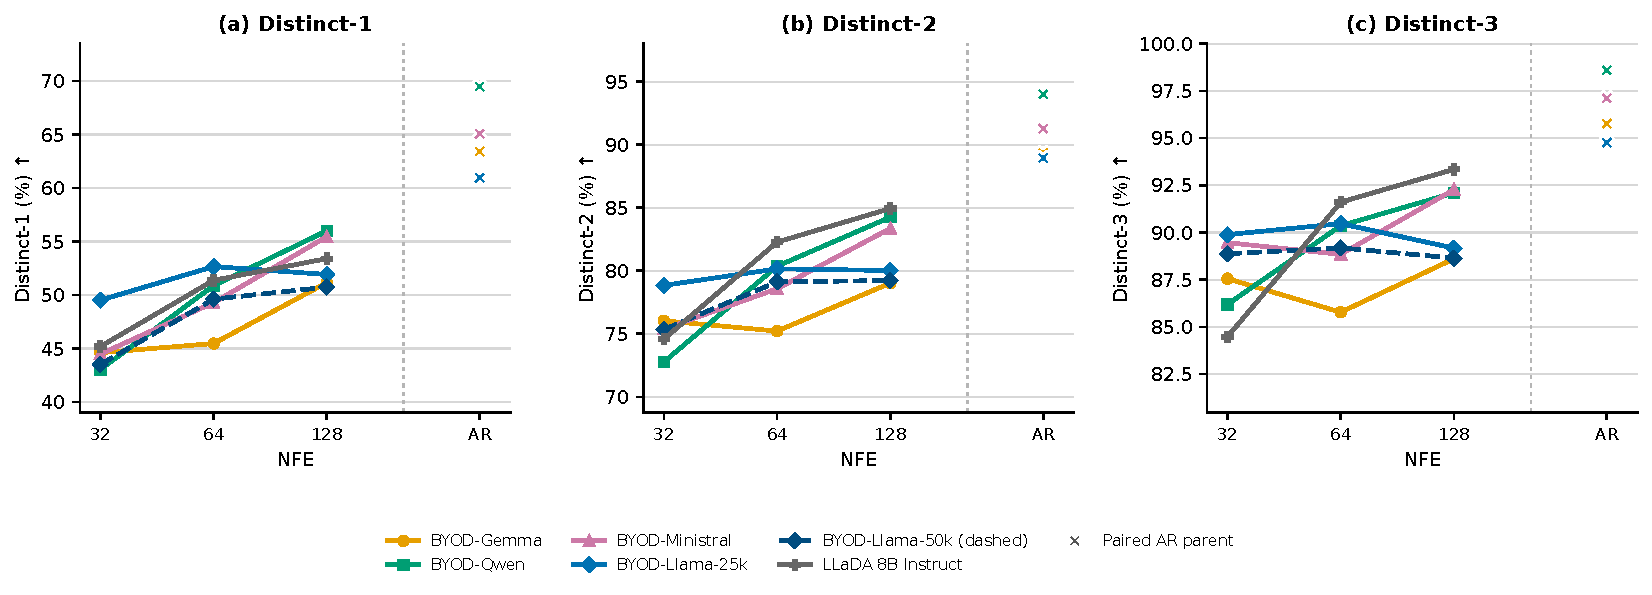
\includegraphics[width=\textwidth]{figures/final_distinct_metrics.pdf}
\caption{Sliding model-token Distinct-1/2/3 for the final models across diffusion inference budgets. Crosses show the paired AR parents; BYOD-Llama-25k and BYOD-Llama-50k share the same parent. Higher-order metrics show the same broad diversity pattern while compressing differences because longer $n$-grams are less likely to repeat exactly.}
\label{fig:final-distinct-metrics}
\end{figure*}

\begin{figure*}[p]
\centering
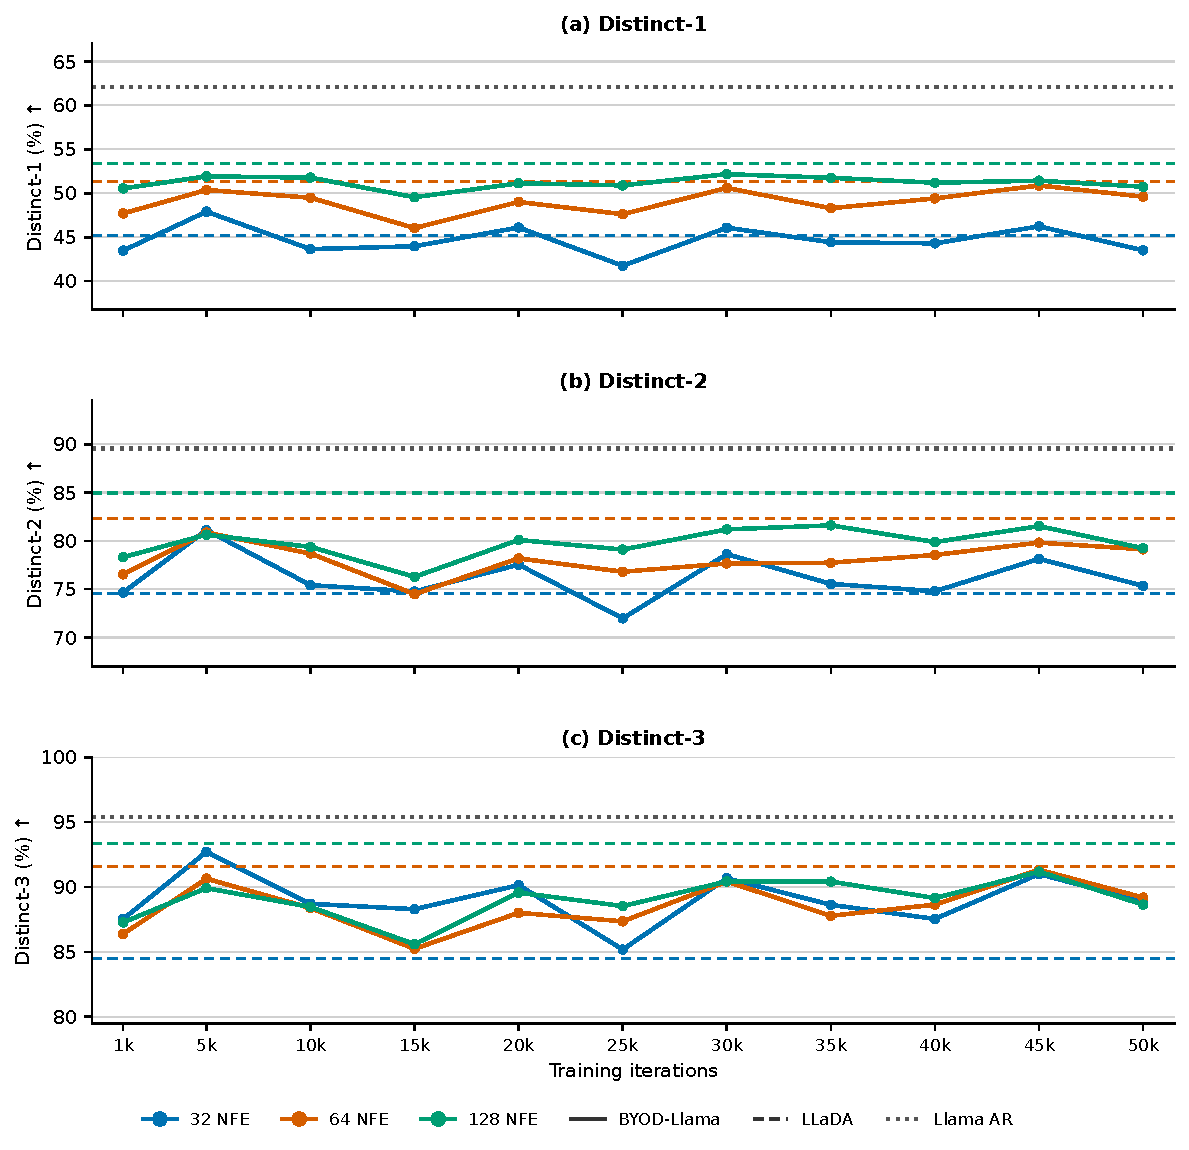
\includegraphics[width=0.92\textwidth]{figures/llama_distinct_progression.pdf}
\caption{Sliding model-token Distinct-1/2/3 throughout BYOD-Llama-50k training. Solid colored lines are BYOD-Llama checkpoints at each NFE budget; matching dashed lines are fixed LLaDA references, and the dotted gray line is Llama AR. All three metrics fluctuate across checkpoints without a strong monotonic trend.}
\label{fig:llama-distinct-progression}
\end{figure*}
\clearpage

\section{Bidirectional attention test}
\label{app:bidirectional-infilling}

This deterministic test uses ordinary single-token target words. Each partial response has the form ``Answer:[MASK]. COPY: apple.'', with a different target in each example. The target is absent from the instruction and left context and appears explicitly after the mask. The converted model predicts the masked position by greedy argmax in one forward pass; no iterative sampling or generation settings are involved.

We score the same masked position twice: once with the later copy clue and once after deleting that clue. We report exact match for both conditions, their difference, and whether adding the clue changes the greedy prediction at all. Under causal attention, changing or deleting tokens to the right cannot affect logits at an earlier position, so both the exact-match gain and prediction-change rate must be zero. The latter separates use of right context from the stricter ability to follow the exact-copy instruction. This is a functional attention check, not a benchmark of reasoning or general infilling quality. Table~\ref{tab:bidirectional-infilling} reports the results for both conditions.

\begin{table}[h]
\caption{Bidirectional attention test results. ``With clue'' predicts the earlier mask while the word is visible later; ``without clue'' removes that later word. Gain is the exact-match difference.}
\label{tab:bidirectional-infilling}
\centering
\scriptsize
\resizebox{\columnwidth}{!}{%
\begin{tabular}{lcccc}
\toprule
Model & With clue EM & Without clue EM & EM gain & Prediction changed \\
\midrule
BYOD-Gemma & 100\% & 0\% & +100 pp & 100\% \\
BYOD-Qwen & 20\% & 0\% & +20 pp & 100\% \\
BYOD-Ministral & 100\% & 0\% & +100 pp & 100\% \\
BYOD-Llama-25k & 90\% & 0\% & +90 pp & 100\% \\
BYOD-Llama-50k & 70\% & 0\% & +70 pp & 100\% \\
LLaDA 8B Instruct & 100\% & 0\% & +100 pp & 100\% \\
\bottomrule
\end{tabular}}
\end{table}

\section{Protocol-separated literature results}
\label{app:published-results}

Table~\ref{tab:published} places our primary Llama conversion beside values reported by other diffusion-model papers \citep{nie2025llada,ye2025dream,nie2026illada,fu2025efficientdlm}. The BYOD column uses our common harness, whereas every other column uses its source paper's evaluation protocol. Differences in prompts, subsets, generation budgets, answer extraction, and execution environments prevent direct ranking; the table is included only to provide scale and task coverage. NR means that the source did not report a value for that task.

\begin{table}[h]
\caption{Our Llama result and protocol-separated published diffusion-model accuracies. Bold marks the largest reported value in each row; it does not imply a controlled comparison. No cross-task averages are shown because task coverage differs by model.}
\label{tab:published}
\centering
\scriptsize
\resizebox{\columnwidth}{!}{%
\begin{tabular}{lccccc}
\toprule
Task & BYOD-Llama (ours) & LLaDA & Dream-Inst. & iLLaDA-Inst. & Efficient-DLM 8B \\
\midrule
ARC-C     & .832 & \textbf{.885} & NR & NR & .619 \\
GPQA      & .296 & \textbf{.333} & .330 & NR & NR \\
GSM8K     & .656 & .694 & .810 & \textbf{.890} & .883 \\
HellaSwag & .704 & \textbf{.746} & NR & NR & .725 \\
HumanEval & .312 & .494 & .555 & .659 & \textbf{.683} \\
MATH      & .256 & .319 & .392 & \textbf{.567} & .501 \\
MBPP      & .432 & .410 & .588 & .580 & \textbf{.610} \\
MMLU      & .592 & .655 & .670 & .716 & \textbf{.772} \\
MMLU-Pro  & .304 & .370 & .433 & \textbf{.523} & NR \\
\bottomrule
\end{tabular}}
\end{table}

\section{Interactive denoising trajectories}
\label{app:demo-trajectories}

Figures~\ref{fig:demo-confidence-trajectories} and~\ref{fig:demo-remasking-trajectories} illustrate how the public BYOD-Gemma demo exposes the parallel refinement process under random and confidence-guided remasking. All panels use the displayed Amsterdam prompt, the helpful-assistant system prompt, temperature 0.7, top-$k$ 3, initial noise fraction 1.0, delayed EOS/EOT retention, permanent locked retention, and no visualization delay. Early stopping is disabled and block length equals the new-token canvas, ensuring that every panel displays its complete denoising budget. The demo randomizes the hidden sampling seed for every request; we resample the 64-NFE conditions to show readable positive examples, so these trajectories illustrate behavior rather than constitute a controlled quality comparison.

\begin{figure*}[p]
\centering
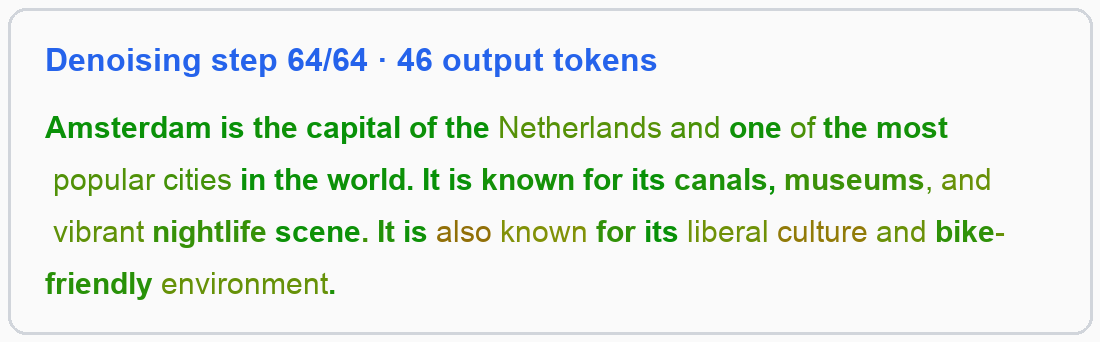
\includegraphics[width=0.67\textwidth]{figures/demo_gemma_confidence_64steps_64tokens_probability.png}
\\[-2pt]\small (a) 64 NFE and 64 tokens.

\vspace{3pt}
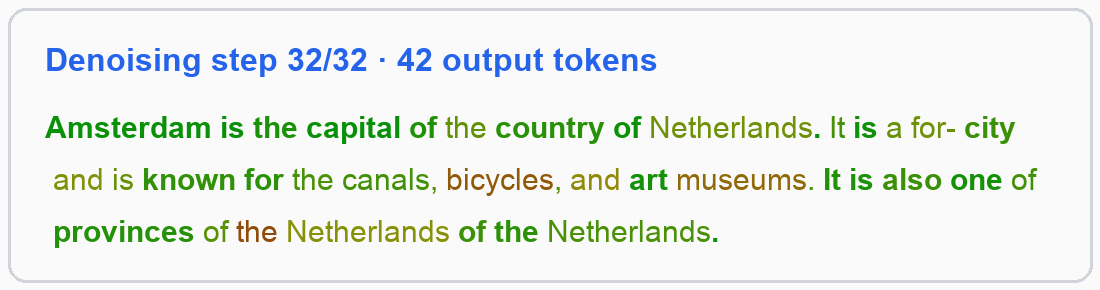
\includegraphics[width=0.67\textwidth]{figures/demo_gemma_confidence_32steps_64tokens_probability.png}
\\[-2pt]\small (b) 32 NFE and 64 tokens.

\vspace{3pt}

\includegraphics[width=0.67\textwidth]{figures/demo_gemma_confidence_16steps_64tokens_probability.png}
\\[-2pt]\small (c) 16 NFE and 64 tokens.
\caption{Confidence-guided BYOD-Gemma-2-9B trajectories at decreasing inference budgets on a 64-token canvas. Red-to-green coloring records each retained token's sampling probability.}
\label{fig:demo-confidence-trajectories}

\vspace{6pt}
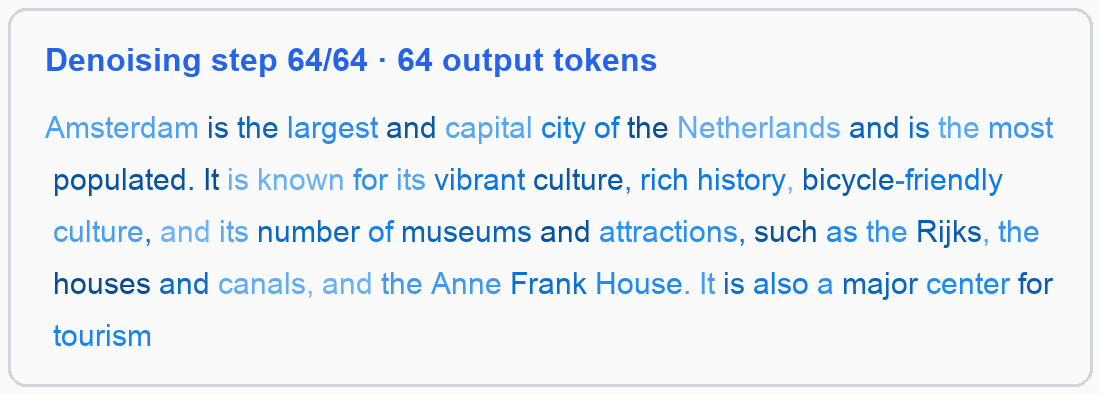
\includegraphics[width=0.67\textwidth]{figures/demo_gemma_random_64steps_64tokens_iteration.png}
\\[-2pt]\small (a) Random remasking; prediction-iteration coloring.

\vspace{3pt}
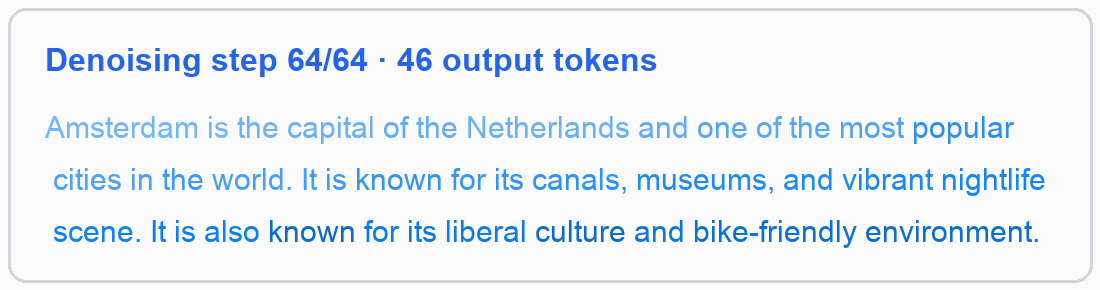
\includegraphics[width=0.67\textwidth]{figures/demo_gemma_confidence_64steps_64tokens_iteration.png}
\\[-2pt]\small (b) Confidence-guided remasking; prediction-iteration coloring.
\caption{Remasking comparison for BYOD-Gemma-2-9B at 64 NFE on a 64-token canvas. Blue intensity records the iteration at which each retained token was predicted.}
\label{fig:demo-remasking-trajectories}
\end{figure*}

\clearpage

\end{document}
